% *****************************************************************************
%
%        FASThesis Manual
%        (FASThesis Class File Documentation)
%
%        Faculty of Applied Sciences
%        University of West Bohemia
%
%        Manual & Explanatory Document
%        Copyright (c) 2022-2024 Kamil Ekštein, Dept. of Computer Science
%        and Engineering, Faculty of Applied Sciences, UWB
%
%        Version:  0.97
%		 Encoding: UTF-8
%		 TeXer:    pdflatex
%
%        Last modification on 22-Apr-2024 by KE
%
% *****************************************************************************

% _____________________________________________________________________________
%
%
%	     DOCUMENT HEADER
%
% _____________________________________________________________________________
%
\documentclass[czech, ma, kiv, he, iso690alph, pdf, viewonly]{fasthesis}
\title{\texttt{FASThesis} -- návod k~použití šablony závěrečné práce na FAV ZČU}
%\worktypespec{Technická zpráva}% <== this command is only applicable if 'oth' switch is used above
\author{Kamil}{Ekštein}{Ing.}{Ph.D.}
\supervisor{Prof. Ing. Tomáš Marný, Ph.D.}
\stagworkid{12345}% <== the unique identifier of the work in the STAG information system
% \auxfrontmattercontent{% <== this command only makes sense if 'oth' switch is used above
	% \section*{Upozornění}%
	% Tento text bude vložen do front matteru\dots
% }
\assignment{zadani.pdf}
\signdate{14}{02}{2024}{V Nové Vsi u~Nového Města na Moravě}% <== the longest local name in the Czech Rep.

\addbibresource{manual.bib}% <== the file with the bibliographical database to be used throughout the text
% _____________________________________________________________________________
%
%
%	     DOCUMENT FRONTMATTER TEXTS
%
% _____________________________________________________________________________
%
\abstract{Text představuje a blíže popisuje třídu (class file) \LaTeX{}ového dokumentu \filename"fasthesis",
která se používá k~sazbě kvalifikačních prací na Fakultě aplikovaných věd Západočeské univerzity v~Plzni. Vysvětluje, jak správně používat šablonu kvalifikační práce \filename"fasthesis" pro sázecí systém \LaTeX{} a jak podobu výsledného dokumentu ovlivňují různé přepínače a příkazy, kterými se sazba při použití této šablony řídí.

Kromě toho, že tento abstrakt skutečně stručně shrnuje obsah dokumentu, tak také slouží jako ukázka, jak by měl abstrakt vypadat. Délka abstraktu by se měla pohybovat mezi 100 a 300 slovy, a ačkoliv není dáno žádné konkrétní omezení, určitě by neměla překročit polovinu stránky A4. Abstrakt má čtenáři poskytnout představu o~tom, co se v~dokumentu dočte (a tedy jestli vůbec má smysl se do čtení pouštět).}
% *** English abstract ***
{The text presents and describes the \LaTeX{} document class \filename"fasthesis", which is used for the typesetting of theses at the Faculty of Applied Sciences, University of West Bohemia in Pilsen. It explains how to properly use the \filename"fasthesis" template for \LaTeX{} typesetting system and how the resulting document is affected by various switches and commands that control the typesetting process when using this template.

Not only this abstract really breifly summarises the document's contents, it also serves as an example of what an abstract might look like. The length of the abstract should be between 100 and 300 words, and although no specific limit is given, it should certainly not exceed half an A4 page. The abstract is intended to give the reader a rough idea of what they will read in the document (and therefore whether it is even worth getting started with it at all).}
\keywords{šablona kvalifikační práce, sazba, DTP, \LaTeX}
% _____________________________________________________________________________
%
%        ACKNOWLEDGEMENT
% _____________________________________________________________________________
%
\acknowledgement{Na tomto místě bych rád poděkoval svému předchůdci v~roli \uv{local wizarda}, člověku,
který připravil první prakticky použitelnou \LaTeX{}ovou šablonu kvalifikační práce na Katedře informatiky
a výpočetní techniky Fakulty aplikovaných věd Západočeské univerzity v~Plzni, Ing. Petru Lobazovi, Ph.D. Asi ještě větší a sr\-deč\-něj\-ší po\-dě\-ko\-vá\-ní si zaslouží úžasný člověk, matematik, který mě s~\TeX{}em před téměř třiceti lety seznámil: Doc. RNDr. František Ježek, CSc.

Rád bych na tomto místě poděkoval i dalšímu matematikovi, Doc. Ing. Janu Pospíšilovi, Ph.D., který mne neúnavně přesvědčoval, že FAV novou šablonu kvalifikačních prací potřebuje jako sůl a následně mě nutil na ní pracovat (a samozřejmě přispěl řadou podnětných připomínek).

Díky si zaslouží i mí drazí kolegové z~Katedry informatiky a výpočetní techniky, kteří svojí konstruktivní
kritikou významně přispěli ke konečné podobě šablony -- jmenovitě jsou to tito (v~abecedním pořadí):
Doc.~Ing.~Přemysl Brada,~M.Sc.,~Ph.D.,
Doc.~Ing.~Pavel Herout,~Ph.D.,
Ing.~Martin Úbl a
Ing.~Petr Vaněček,~Ph.D.

Zvláštní poděkování pak patří Ing.~Františku Pártlovi, který šablonu intenzivně testoval, pomáhal opravovat chyby, neúnavně se staral o gitový repozitář šablony (což bylo s ohledem na můj vztah ke gitu zvláště náročné) a zejména zajišťoval integraci šablony do Overleafu.

V~neposlední řadě si poděkování zaslouží také studenti, kteří aktivně pomáhali při testování nově vzniklé šablony: Bc.~Veronika Báčová a Petra Ocelíková.
\begin{flushright}
\textit{Kamil Ekštein},\\
autor šablony\\
(únor 2024)
\end{flushright}
}
% _____________________________________________________________________________
%
%        ADDITIONAL FRONT MATTER CONTENT
% _____________________________________________________________________________
\auxfrontmattercontent{%
\section*{Note for English readers}
\fbox{\parbox[t]{\textwidth}{\textbf{%
In case that your command of the Czech language is not sufficient for a perfect understanding of the whole of this document, please be so kind and open the file \filename"manual_en.pdf" which contains the same text (i.e. the user's manual for the \LaTeX{} template \filename"fasthesis.cls") in English.
}}}}
% _____________________________________________________________________________
%
%
%	     DOCUMENT TEXT BEGINNING
%
% _____________________________________________________________________________
%
\begin{document}
\frontpages[tm] % or notm if the `trademark' declaration is not needed
\tableofcontents
% 
% -x---- ADDITIONAL COLOUR DEFINITIONS ----------------------------------------
%
\makeatletter%
\ifx\FASThesis@style\c@fullcolor%
	\definecolor{fascolor}{cmyk}{0.06, 0.27, 1.0, 0.12}%
	\definecolor{fascolordk}{cmyk}{0.05, 0.28, 1.0, 0.24}%
\else%
	\definecolor{fascolor}{cmyk}{0, 0, 0, 0.6}%
	\definecolor{fascolordk}{cmyk}{0, 0, 0, 0.75}%
\fi%
\makeatother%
\lstdefinestyle{plainsrc}{
	backgroundcolor=\color{fascolor!10},
	basicstyle=\ttfamily\footnotesize,
	numberstyle=\tiny\color{fascolordk},
	numbers=left,
	numbersep=5pt,
	keepspaces=true,
	tabsize=2,
	extendedchars=true,
	literate={á}{{\'a}}1 {č}{{\v{c}}}1 {ď}{{\v{d}}}1 {é}{{\'e}}1 {ě}{{\v{e}}}1 {è}{{\`{e}}}1 {í}{{\'{\i}}}1 {ľ}{{\v{l}}}1 {ň}{{\v{n}}}1 {ó}{{\'o}}1 {ŕ}{{\'r}}1 {ř}{{\v{r}}}1 {š}{{\v{s}}}1 {ť}{{\v{t}}}1 {ú}{{\'u}}1 {ů}{{\r{u}}}1 {ý}{{\'y}}1 {ž}{{\v{z}}}1
	{Á}{{\'A}}1 {Č}{{\v{C}}}1 {Ď}{{\v{D}}}1 {É}{{\'E}}1 {Ě}{{\v{E}}}1 {È}{{\`{E}}}1 {Í}{{\'I}}1 {Ľ}{{\v{L}}}1 {Ň}{{\v{N}}}1 {Ó}{{\'O}}1 {Ŕ}{{\'R}}1 {Ř}{{\v{R}}}1 {Š}{{\v{S}}}1 {Ť}{{\v{T}}}1 {Ú}{{\'U}}1 {Ů}{{\r{U}}}1 {Ý}{{\'Y}}1 {Ž}{{\v{Z}}}1
}
% -x---- END OF ADDITIONAL COLOUR DEFINITIONS ---------------------------------
% _____________________________________________________________________________
%
%
%        CHAPTER
%
% _____________________________________________________________________________
%
\chapter*[Předmluva]{Předmluva}
Milý autore/milá autorko,\\[\baselineskip]
tímto se do Vašich schopných rukou dostává \term{šablona kvalifikační práce} na Fakultě aplikovaných věd Západočeské univerzity v~Plzni. Tato šablona je určena k~dosažení jednotného vzhledu kvalifikačních prací sázených v~typografickém systému \LaTeX. Při jejím návrhu jsem se řídil zejména tím, aby bylo její používání pro (často ne\-zku\-še\-né\-ho) autora textu co nejsnazší, ale aby zároveň výsledný produkt odpovídal zásadám a pravidlům moderní sazby technických dokumentů, působil dostatečně reprezentativně a zároveň lehce a přirozeně, a přitom byl přehledný a dobře čitelný. Grafická podoba šablony pak reflektuje pravidla stanovená \term{Manuálem jednotného vizuálního stylu} Západočeské univerzity v~Plzni\footnote{Z tohoto manuálu vychází kromě podoby logotypů univerzity a jejích součástí zejména barevnost a použití konkrétních fontů.}.

Při tvorbě šablony jsem vycházel z~obdobných šablon, které jsou autorům kvalifikačních prací k~dispozici na významných českých i zahraničních vysokých školách. Snažil jsem se je důkladně analyzovat, abych \uv{to dobré} začlenil i do naší šablony, a naopak \uv{tomu špatnému} abych se vyhnul. Grafické a typografické prvky, vyskytující se v~těchto šablonách, jsem hodnotil na základě poznatků čerpaných ze tří skvělých knih: Graphic Design Now~\cite{Fiells2005} od Charlotte a Petera Fiellových, Jazyk grafického designu~\cite{Poulin2012} od Richarda Poulina a Typografický manuál~\cite{Beran2016} od Vladimíra Berana.

Výše popsaným způsobem šablonu ovlivnily šablony kvalifikačních prací \emph{Kalifornského technologického institutu} (Caltech), \emph{Harvardovy univerzity}, \emph{Princetonské univerzity}, \emph{Newyorské univerzity}, \emph{Univerzity v~Oslu}, \emph{Vysokého učení technického v~Brně}, \emph{Matematicko-fyzikální fakulty Univerzity Karlovy}, \emph{Fakulty informatiky Masarykovy univerzity} a řada dalších. Důležitou roli pochopitelně sehrála i naše předchozí \LaTeX{}\-ová šablona, připravená před řadou let Petrem Lobazem.

Tato šablona by měla řešit prakticky všechny zásadní aspekty sazby kvalifikační práce (a pokud je přímo neřeší, vždy je možné je řešit ve vlastní režii použitím příkazů \TeX{}u), nicméně -- protože je zatím (v~únoru 2024) docela nová a \uv{nezajetá} -- může se stát, že v~ní odhalíte chybu, nedostatek, nějaké nekonzistentní chování apod. Pokud se tak stane, budu rád, když mi napíšete, o~co jde a jak se problém projevuje, e-mailem na adresu \url{kekstein@kiv.zcu.cz} a já se pokusím zajistit co možná nejdříve nápravu. Někdy se ovšem může jednat o~situaci, kterou programátoři popisují obvykle (v~anglickém originále) větou: \uv{It's not a bug, it's a feature.}

Doufám, že se Vám s~touto šablonou bude pracovat dobře a pomůže Vám vytvořit perfektní kvalifikační práci, která bude následně úspěšně obhájena. K~tomu Vám přeju z~pozice jejího tvůrce hodně štěstí a držím palce.
% _____________________________________________________________________________
%
%
%        CHAPTER
%
% _____________________________________________________________________________
%
\chapter{Úvod}
Tato \term{šablona kvalifikační práce} nastavuje převážnou většinu parametrů sazby v~typografickém systému \LaTeX{} tak, aby výsledný dokument odpovídal jednak požadavkům norem (pokud existují) a jednak tradičním zvyklostem úpravy vědecko-technických dokumentů. Je navržena tak, aby nebylo nutné žádné parametry sazby \uv{ručně} upravovat. Zkušení uživatelé \LaTeX{}u nicméně pochopitelně mohou vzhled sazby snadno změnit použitím příkazů \LaTeX{}u a maker, která poskytuje základní třída dokumentu využitá v~této šabloně. Zejména z~tohoto důvodu -- pro zkušené uživatele -- je tedy dobré vědět, že
\begin{center}
\framebox{třída \filename"fasthesis" této šablony je založena na třídě \filename"memoir".}
\end{center}
Lze tedy používat kompletní aparát třídy \filename"memoir"~\cite{memoir}, je-li to vhodné (ovšem není to vůbec nutné).

Šablona ovlivňuje zásadním způsobem vzhled výsledného dokumentu tak, aby jednak jasně deklaroval příslušnost k~Fakultě aplikovaných věd Západočeské univerzity v~Plzni\footnote{Šablona je k~dispozici jako open source, a je tedy možné ji libovolně modifikovat za podmínky dodržení ustanovení licence LGPL. Pokud tedy nejste z~FAV ZČU a chcete tuto šablonu použít, směle do toho: Bude zřejmě třeba změnit barevnost a zejména \textbf{font!} Proč? Použitý bezpatkový font nadpisů \emph{GT America} není volně k~dispozici -- ZČU je vlastníkem komerční licence na jeho použití, neboť je nedílnou součástí jejího vizuálního stylu. Jste-li tedy z~jiné instituce, která nemá tento font zakoupený, použít jej nemůžete a je \textbf{nutné} jej nahradit jiným (doporučuji třeba volně dostupný font \emph{Roboto Condensed}).}, druhak aby byl text přehledný a dobře čitelný a aby bylo pokud možno \uv{o~vše postaráno} automaticky a autor nemusel řešit např. vzhled a provedení citací použité literatury, umístění a přesné znění prohlášení atp.
%
%
%
\section{Instalace}
Šablonu není nutné  na váš počítač vůbec instalovat (stejně jako celý \TeX) v~případě, že hodláte k~sepsání kvalifikační práce využít online editor \term{Overleaf} -- na adrese URL \url{https://www.overleaf.com/read/ryhpnsmtgrrs} je šablona pro tento editor již k~dispozici, připravena k~okamžitému použití. Pro studenty FAV ZČU se pak nabízí ještě lepší možnost, a to využít lokální instalace Overleafu/Share\LaTeX{}u na serveru Katedry informatiky a výpočetní techniky FAV ZČU na adrese URL \url{https://overleaf.kiv.zcu.cz} -- tam se totiž neuplatňuje omezení na čas kompilace dokumentu jako v případě zdarma dostupného Overleafu.

Pokud ovšem používáte \TeX{} pravidelně a máte jej tedy nainstalovaný na svém počítači (což je silně \textbf{doporučená} varianta), není instalace šablony také nijak komplikovaná. Postupujte podle krok za krokem podle níže uvedeného návodu:
\begin{enumerate}
\item Stáhněte si instalační archiv \filename"fasthesis.zip".
\item \textbf{Vytvořte} pro projekt (tedy vaši kvalifikační práci) \textbf{samostatnou složku/adresář}.
\item Do vytvořené složky \textbf{nakopírujte} ze staženého instalačního archivu \textbf{soubor} \filename"fasthesis.cls" -- to je základní a nejdůležitější soubor, kterým je šablona tvořena -- definice třídy dokumentu \filename"fasthesis".
\item Dále do vytvořené složky \textbf{zkopírujte jako podsložku složku \filename"img"} -- v~té se nacházejí obrázky, které šablona využívá (zejména loga fakulty a kateder a tématické grafické motivy na titulní stránku).
\item Do složky pak \textbf{také uložte zadání vaší kvalifikační práce ve formátu PDF}, lhostejno, zda je naskenované nebo vygenerované informačním systémem univerzity. Na názvu tohoto PDF souboru nezáleží, do dokumentu je zadání vloženo příkazem \verb"\assignment{zadani.pdf}", jehož parametrem je právě tento název (může být i s~cestou do nějaké podsložky).
\item Nakonec je třeba nainstalovat font \emph{GT America}, který je předepsán \term{Manuálem jednotného vizuálního stylu} Západočeské univerzity v~Plzni jako font nadpisů. Tuto netriviální akci popisuje detailně příloha \ref{app:installgta}.

Pokud by informace z~přílohy \ref{app:installgta} nebyly dostatečně úplné a instalace fontů by vám činila problémy, využijte stránky organizace TUG (= \textit{\TeX{} Users' Group}), které se tématu instalace fontů věnují -- najdete je na URL \url{https://tug.org/fonts/fontinstall.html}.
\end{enumerate}
% _____________________________________________________________________________
%
%
%        CHAPTER
%
% _____________________________________________________________________________
%
\chapter{Použití šablony}
Šablonu tvoří (kromě jiného) zejména soubor definice třídy \LaTeX{}ového dokumentu, tzv. \term{classfile}, nazvaný \filename"fasthesis.cls", který \LaTeX{}u poskytuje třídu dokumentu \filename"fasthesis".

Zdrojový text vaší práce tedy je obyčejný textový soubor (v~kódování UTF-8\footnote{Je sice možné celkem snadno šablonu \uv{překódovat} do jiného kódování znaků národních abeced, ale při současném stavu užívání různých operačních systémů, editorů a dalších podpůrných nástrojů se to nejeví jako rozumné.}), jehož úvodním příkazem je \verb"\documentclass{fasthesis}". Jeho detailní nastavení prostřednictvím nepovinných parametrů bude popsáno dále.
%
%
%
\section{Nastavení třídy \texttt{fasthesis}}
Třída dokumentu \filename"fasthesis" má celou řadu \uv{přepínačů}, tedy nepovinných parametrů, které ovlivňují, jak bude výsledný dokument vypadat. Základní nastavení odpovídá použití příkazu v~této podobě:
\lstset{style=plainsrc, numbers=none}
\begin{lstlisting}
\documentclass[czech, kiv, ba, he, iso690alph, pdf]{fasthesis}
\end{lstlisting}
Výsledný dokument tedy bude vysázen v~českém jazyce (``\verb"czech"''), bude použito logo a označení Katedry informatiky a výpočetní techniky (``\verb"kiv"''), nadpis na titulní straně (a jinde) uvede práci jako bakalářskou kvalifikační práci (``\verb"bc"''), jejím autorem je osoba používající pro sebe osobní zájmeno \uv{on} (``\verb"he"''), bibliografické informace budou formátovány podle
normy ISO ČSN 690 (``\verb"iso690alph"'') v~podobě doporučené např. webem \texttt{https://www.citace.com} nebo \texttt{https://citace.zcu.cz}, přičemž zdroje budou v~textu identifikovány zkratkou jména autora (či prvními písmeny jmen autorů, je-li jich více) a posledními dvěma číslicemi roku vydání publikace (např. [AB2023]).
%interních pravidel šablony
%\footnote{Tato pravidla \textbf{jsou v naprosté shodě s ustanoveními ČSN ISO 690}, ale formátování položek seznamu literatury je mírně odlišné od podoby doporučené např. webem {\ttfamily\footnotesize https://www.citace.com} nebo {\ttfamily\footnotesize https://citace.zcu.cz}.}
%(``\verb"ftalph"'')
Finální produkt sazby bude používán zejména online v~podobě dokumentu ve formátu PDF (``\verb"pdf"'') nebo bude vytištěn na kvalitní barevné tiskárně -- nepředpokládá se tedy primárně tisk dokumentu na černobílé tiskárně.
%
%
%
\subsection{Seznam přepínačů třídy \texttt{fas\-the\-sis}}
Tabulka \ref{tab:allclassoptions} na str. \pageref{tab:allclassoptions} přehledně shrnuje všechny použitelné přepínače, které ovlivňují chování šablony. Některé z~nich se (pochopitelně) navzájem vylučují (např. ``\verb"he"'' a ``\verb"she"'') a jsou-li užity současně, buď se provede pouze poslední z~nich, nebo se dokument dokonce může začít chovat podivně (neměl by, ale kdo ví).
%
\begin{center}
\begin{longtable}{p{.15\textwidth}p{.7\textwidth}}
\caption{Seznam všech použitelných přepínačů třídy dokumentu {\ttfamily fasthesis}}
\label{tab:allclassoptions}\\
\toprule[1.5pt]
\textbf{přepínač} & \textbf{vysvětlení}\\
\midrule
\endfirsthead
\multicolumn{2}{c}{\tablename{}~\thetable{} \textit{(pokračování z~předchozí stránky)}}\\
\midrule
\textbf{přepínač} & \textbf{vysvětlení}\\
\midrule
\endhead
\midrule
\multicolumn{2}{r}{\textit{(tabulka pokračuje na další stránce)}}\\
\endfoot
\bottomrule[1.5pt]
\endlastfoot
%
\verb"czech" & Dokument bude sázen v~českém jazyce, budou použity české verze log a názvů univerzity a jejích součástí, v~češtině budou všechny automaticky vkládané texty (prohlášení apod.), české bude dělení slov v~dokumentu atp.\\
\verb"english" & Dokument bude sázen v~anglickém jazyce, budou použity anglické verze log a názvů univerzity a jejích součástí, v~angličtině budou všechny automaticky vkládané texty (prohlášení apod.), anglické bude dělení slov v~dokumentu atp.\\
\midrule
\verb"he" & Text píše osoba používající pro sebe osobní zájmeno \uv{on}.\\
\verb"she" & Text píše osoba používající pro sebe osobní zájmeno \uv{ona}.\\
\midrule
\verb"sem" & Dokument je seminární práce.\\
\verb"ba" & Dokument je bakalářská kvalifikační práce.\\
\verb"bc" & Dokument je bakalářská kvalifikační práce (\textit{alias přepínače} ``\verb"ba"'').\\
\verb"ma" & Dokument je diplomová, tj. magisterská kvalifikační práce.\\
\verb"mgr" & Dokument je diplomová, tj. magisterská kvalifikační práce (\textit{alias přepínače} ``\verb"ma"'').\\
\verb"ing" & Dokument je diplomová, tj. magisterská kvalifikační práce (\textit{alias přepínače} ``\verb"ma"'').\\
\verb"ddt" & Dokument je rigorózní práce (= \textit{doctoral dissertation theses}).\\
\verb"rig" & Dokument je rigorózní práce (\textit{alias přepínače} ``\verb"ddt"'').\\
\verb"phd" & Dokument je doktorská disertační práce.\\
\verb"hab" & Dokument je habilitační práce.\\
\verb"oth" & Dokument je něco jiného (= \textit{other}) a z~výše uvedených možností si nelze vybrat. V~tomto případě je pak nutné dodatečně nastavit některé parametry šablony použitím k~tomu určených příkazů, viz sekce \ref{sec:otherworktype} na str. \pageref{sec:otherworktype}.\\
\midrule
\verb"kgm" & Práce je odevzdávána na Katedře geomatiky.\\
\verb"kfy" & Práce je odevzdávána na Katedře fyziky.\\
\verb"kiv" & Práce je odevzdávána na Katedře informatiky a výpočetní techniky.\\
\verb"kma" & Práce je odevzdávána na Katedře matematiky.\\
\verb"kme" & Práce je odevzdávána na Katedře mechaniky.\\
\verb"kky" & Práce je odevzdávána na Katedře kybernetiky.\\
\midrule
\verb"ftalph" & Formátování bibliografických informací je provedeno podle interních pravidel šablony (ve shodě s~normou ČSN ISO 690).\\
\verb"iso690numb" & Formátování bibliografických informací je provedeno tak, jak doporučuje norma ČSN ISO 690 a některé organizace či iniciativy, zabývající se etikou vědeckého výzkumu a specificky správným citováním (např. weby \url{https://www.citace.com} či \uv{náš} \url{https://citace.zcu.cz}), přičemž jednotlivé zdroje jsou pak označeny vzestupně čísly, např. takto: [1], [2], [3].\\
\verb"iso690alph" & Shodné s~``\verb"iso690numb"'', ale jednotlivé zdroje jsou označeny zkratkou jména autora či prvních písmen jmen autorů a posledními dvěma číslicemi roku vydání publikace, např. takto: [Kra19], [ČM23].\\
\verb"iso690auyr" & Shodné s~``\verb"iso690numb"'', ale jednotlivé zdroje jsou označeny jmény autorů a datem vydání publikace, např. takto: (Král, 2019), (Čáp; Mák, 2023).\\
\midrule
\verb"pdf" & Dokument je určen primárně k~uložení a prohlížení online ve formátu PDF, je tedy vysázen barevně a s~grafickými motivy.\\
\verb"prn" & Dokument je určen primárně k~tisku na černobílé tiskárně, tzn. nebude vysázen s~barevnými (typo)grafickými motivy a grafikou na pozadí titulní stránky.\\
\verb"nobggfx" & Dokument bude vysázen barevně, ale bez grafického motivu na pozadí titulní stránky (\textit{= no background graphics}).\\
\verb"viewonly" & Dokument je určen \textbf{pouze pro prohlížení} na obrazovce počítače -- nebude tištěn. Neobsahuje proto prázdné sudé stránky na jednostranně potištěných listech (pro pokročilé \TeX{}isty: odpovídá přepínači ``\verb"oneside"'' standardních \LaTeX{}ových tříd \verb"book", \verb"report" atp., a samozřejmě také použité základní třídy \verb"memoir").\\
\end{longtable}
\end{center}
%
%
%
%
\section{Minimální kostra dokumentu třídy {\ttfamily fas\-the\-sis}}
\LaTeX{}ový kód níže ukazuje základní, nejjednodušší použití třídy {\ttfamily fas\-the\-sis} pro sazbu dokumentu. Některé příkazy \emph{není nutné} použít, resp. nezpůsobí to chybu při zpracování dokumentu \LaTeX{}em, ale v~takovém případě se vysázejí kódem šablony přednastavené hodnoty, což by ve skutečné kvalifikační práci mohlo být docela na závadu.
%
\lstset{style=plainsrc}
\begin{lstlisting}
\documentclass[czech, ing, kiv, he]{fasthesis}
\title{\texttt{FASThesis} -- návod k~použití šablony zá...}
\author{Kamil}{Ekštein}{Ing.}{Ph.D.}
\supervisor{Prof. Ing. Tomáš Marný, Ph.D.}
\stagworkid{12345}
\assignment{zadani.pdf}
\signdate{31}{12}{2022}{V Nové Vsi u~Nového Města na Moravě}
\addbibresource{manual.bib}
\abstract{Text abstraktu v~jazyce práce, tj. zde česky.}
{The abstract text in a secondary language, here in English.}
\keywords{šablona kvalifikační práce, sazba, DTP, \LaTeX}
\acknowledgement{Text poděkování.}
\begin{document}
\frontpages[tm]
\tableofcontents
\chapter{Úvod}
...
\appendix
\chapter{První příloha}
...
\backmatter
\printbibliography
\backpage
\end{document}
\end{lstlisting}
%
Úvodní (\uv{stavové}) příkazy před příkazem \verb"\begin{document}" je samozřejmě možné uvést v~libovolném pořadí, protože sazba textu podle jimi nastavených hodnot se provede najednou až vydáním příkazu \verb"\frontpages".
%
%
%
%
\section{Některé úvodní \uv{stavové} příkazy}
Většina úvodních příkazů, nastavujících zejména texty v~tzv. \emph{front matteru} (jako je např. titul, patitul, různá prohlášení apod.), je \uv{samovysvětlující} -- podívejte se do zdrojového kódu tohoto manuálu (který je součástí distribučního balíčku) a mělo by být jasno. Dále tedy budou uvedeny pouze ty příkazy, které v~sobě skrývají nějaké záludnosti.
%
%
%
\subsection{Nastavení jména autora práce}
\label{sec:authorsname}
Zatímco u~běžně používaných \LaTeX{}ových tříd (\filename{article}, \filename{report}, \filename{book} apod.) i u~základní třídy \filename{memoir} má příkaz \verb"\author{"\textsl{jméno autora}\verb"}" pouze jediný argument, kterým je jméno autora (míněno celé jméno, včetně křestních a dalších jmen a případných titulů) v~takové podobě, v~jaké si ho autor přeje vysázet na titulní stránku, u~této šablony (tedy třídy \filename{fasthesis}) je situace složitější:

Z~řady technických důvodů je nutné, aby šablona \uv{znala} i jednotlivé komponenty jména. Proto má modifikovaný příkaz \verb"\author" v~dokumentu třídy \filename{fasthesis} podobu \verb"\author{"\textsl{křestní jméno}\verb"}{"\textsl{příjmení}\verb"}{"\textsl{tituly před jménem}\verb"}{"\textsl{tituly za jménem}\verb"}" -- tedy celkem 4 \textbf{povinné} argumenty.

Ač třeba v~okamžiku, kdy píšete např. diplomovou práci, ještě nemáte titul(y) za jménem, není možné některý z~argumentů vynechat. Všechny 4 argumenty musí být uvedeny, ale některé mohou být samozřejmě prázdné:
%
\lstset{style=plainsrc, numbers=none}
\begin{lstlisting}
\author{Jan}{Novák}{Bc.}{}
\end{lstlisting}
%
%
%
%
\subsection{Nastavení identifikačního čísla práce v~informačním systému ZČU STAG}
\label{sec:stagworkid}
V~informačním systému STAG, který používá ZČU (a řada jiných univerzit), jsou všechny kvalifikační práce (nejen odevzdané a obhájené, ale i rozpracované) uloženy pod \emph{unikátním číselným identifikátorem}, který dovoluje práci zobrazit (je-li správně použit v~konkrétním URL) a případně i stáhnout ve formátu PDF.

Tento unikátní identifikátor práce je možné šabloně předat příkazem \verb"\"\texttt{stag\-work\-id\{}\textsl{identifikátor práce}\verb"}", načež šablona zajistí jeho zakódování do QR kódu, který pak (pokud si to autor přeje) lze umístit na zadní stranu desek práce jako součást grafického motivu (detailně popsáno v~sekci \ref{sec:lastpage} na straně \pageref{sec:lastpage}). Užití ukazuje příklad:
%
\lstset{style=plainsrc}
\begin{lstlisting}
\documentclass[czech, ma, kiv, he, pdf]{fasthesis}
\title{\texttt{FASThesis} -- návod k~použití šablony ...}
\author{Kamil}{Ekštein}{Ing.}{Ph.D.}
\supervisor{Prof. Ing. Tomáš Marný, Ph.D.}
\stagworkid{12345}
\assignment{zadani.pdf}
\signdate{14}{02}{2024}{V Nové Vsi u~Nového Města na Moravě}
\begin{document}
\frontpages[tm]
...
(TEXT PRÁCE)
...
\backmatter
\setbackpageqrcode
\backpage
\end{document}
\end{lstlisting}
%
Jak ve STAGu nalézt předmětný unikátní identifikátor práce je popsáno poznámce pod čarou \ref{tpos:workid} na straně \pageref{tpos:workid}.
%
%
%
\subsection{Vložení zadání kvalifikační práce}
Zadání kvalifikační práce (tak jak je uloženo ve STAGu) se do dokumentu vkládá příkazem \verb"\assignment{"\textsl{jméno souboru}\verb"}". Toto zadání je třeba nejprve ze STAGu \textbf{vyexportovat ve formátu PDF} a uložit do složky, ve které je zdrojový kód dokumentu kvalifikační práce (v~případě práce v~Overleafu pak do kořenové složky projektu, \uv{vedle} samotného \TeX{}ového zdrojového kódu dokumentu).

Soubor PDF se zadáním může být uložen i v~nějaké podsložce. Je-li tomu tak, musí být uvedena celá relativní cesta k~tomuto souboru (i v~případě Windows uvádějte v~cestě \textbf{lomítka normální}, nikoliv zpětná), tj. např.:
%
\lstset{style=plainsrc, numbers=none}
\begin{lstlisting}
\assignment{vloz/dokumenty/zadani.pdf}
\end{lstlisting}
%
\textbf{Upozornění:} Ze specifikovaného souboru ve formátu PDF se vloží do výsledného dokumentu \emph{nejvýše první dvě stránky} (což by mělo stačit a mělo by to být správně, pokud je v~PDF skutečně zadání kvalifikační práce -- to je na FAV totiž vždy jedno- nebo dvojstránkové).
%
%
%
\subsection{Specifikace souboru s~bibliografickou databází}
Bibliografické informace v~dokumentu třídy \filename"fasthesis" spravuje kombinace nástroje \filename"biber" a balíku \filename"biblatex". Zkušenější uživatelé \TeX{}u se mohou ptát, proč šablona opouští léty prověřený nástroj \filename"bibtex" s~možností ovlivnit vzhled sazby bibliografických informací prostřednictvím souboru \filename".bst" (\textit{= bibliography style}). Je to proto, že \filename"bibtex" nepracuje korektně se znaky národních abeced kódovanými v~rozšířených kódováních UTF-8 apod. Backend \filename"biber" je o~dost novější, takže s~tím problémy nemá.

Mechanismus \filename"biber" + \filename"biblatex" vyžaduje, aby již na začátku dokumentu byl specifikován soubor, ve kterém se nachází bibliografická databáze. To se provádí příkazem \verb"\addbibresource{"\textsl{soubor s~bibliografickou databází}\verb"}", takže třeba takto:
%
\lstset{style=plainsrc, numbers=none}
\begin{lstlisting}
\addbibresource{moje_literatura.bib}
\end{lstlisting}
%
Obsah souboru \filename".bib" -- tedy bibliografická databáze sázeného dokumentu -- je stejný, jako tomu bylo v~případě \filename"bibtex"u. Používá se stejná syntax a totožné formátování, tzn. pokud již autor má z~dřívějška vlastní bibliografickou databázi ve formátu \filename"bibtex", kterou si např. budoval v~průběhu studia při psaní různých prací, může ji bez úprav okamžitě použít.

Ukázka níže zobrazuje typickou podobu úseku souboru \filename".bib" s~jedním konkrétním bibliografickým záznamem typu \emph{kniha}:
%
\lstset{style=plainsrc}
\begin{lstlisting}
@book{Poulin2012,
	title="Jazyk grafického designu",
	author="Richard Poulin",
	publisher="Slovart",
	year="2012",
	address="Praha",
	isbn="978-80-7391-552-0"
}
\end{lstlisting}
%
Na takovýto záznam se pak v~textu odkazuje pomocí příkazů \TeX{}u \verb"\cite{"\textsl{identifikátor zdroje}\verb"}":
%
\lstset{style=plainsrc}
\begin{lstlisting}
... najdeme např. ve vynikající knize Jazyk grafického
designu~\cite{Poulin2012}, která ...
\end{lstlisting}
%
K~dalším specifickým způsobům citací zdrojů lze pak využít příkazy \verb"\citep{...}", \verb"\citet{...}" atp. z~balíku \filename"natbib"; detaily jsou popsány např. na adrese URL \url{https://en.wikibooks.org/wiki/LaTeX/Bibliography_Management}.

Zásadní výhodou použitého formátu \filename"bibtex" je fakt, že je de facto standardem v~oblasti přírodovědných a vědecko-technických publikací, a tedy drtivá většina online služeb pro vyhledávání zdrojů informací (jako je např. \term{Google Scholar}, \term{IEEE Xplore}, \term{Web of Science}, \term{Scopus} atd.) umí citační záznamy v~tomto formátu přímo generovat.

Úplný popis formátu \filename"bibtex" pro vedení bibliografických databází pak může autor kvalifikační práce najít na webu věnovaném nástroji \filename"bibtex" na adrese URL \url{https://www.bibtex.com/g/bibtex-format/}.
%
%
%
\subsection{Abstrakt}
K~sazbě abstraktu práce slouží příkaz \verb"\abstract{"\textsl{textu abstraktu v~jazyce práce}\verb"}{"\textsl{text abstraktu ve zvoleném cizím jazyce}\verb"}". Píše-li tedy autor práci česky, bude v~prvním argumentu příkazu celý text abstraktu v~češtině, ve druhém argumentu pak celý text abstraktu přeložený do cizího jazyka, v~našem oboru to patrně bude téměř vždy angličtina. Píše-li však autor kvalifikační práci \textbf{anglicky}, bude prvním argumentem \textbf{anglicky psaný abstrakt} práce a ve druhém argumentu bude odpovídající text \textbf{česky} (tady už se možnost volby nenabízí, protože kvalifikační práce je odevzdávána v~Česku, na české vysoké škole). Výjimku z~tohoto pravidla může mít pouze cizinec píšící kvalifikační práci anglicky, který pak pro text druhého argumentu použije svůj rodný jazyk (není-li jím angličtina).

Ve druhé popsané variantě příběhu s~abstraktem by ovšem došlo k~nepříjemné situaci, kdy bude text abstraktu v~rodném jazyce cizince nadepsán česky (protože příkaz \verb"\abstract" za normálních okolností používá pro nadpisy abstraktů pouze český výraz \uv{Abstrakt} a jeho anglický ekvivalent \uv{Abstract}). Právě proto, aby šla tato nežádoucí eventualita vyloučit, lze použít příkaz \verb"\abstract" s~nepovinným parametrem, kterým je správná podoba nadpisu cizojazyčného abstraktu. Ukázka níže předvádí, jak by vypadal např. abstrakt práce psané anglicky autorem, jehož rodnou řečí je francouzština:
%
\lstset{style=plainsrc}
\begin{lstlisting}
\abstract[Résumé]{This thesis describes the effect of ...}
  {Cette thèse décrit l'effet de ...}
\end{lstlisting}
%
%
%
\subsection{Klíčová slova}
Klíčová slova se do dokumentu vkládají příkazem \verb"\keywords{"\textsl{seznam klíčových slov oddělených čárkami}\verb"}". Klíčových slov by nemělo být moc, optimální počet je obvykle někde mezi 3 a 8 (ale není to dogma, počet se může samozřejmě lišit např. podle složitosti a rozsahu pojednávané problematiky).

Píše-li autor práci česky, uvádí se jednotlivá klíčová slova (i slovní spojení) \textbf{s~malými počátečními písmeny} (všech slov ve spojení, pokud to nejsou vlastní jména či názvy produktů apod.). Naopak v~angličtině se obvykle tzv. kapitalizují, tedy počáteční písmena slov (prvních slov ve slovních spojeních) se píšou velká.

V~případě práce psané v~češtině, a tedy českých klíčových slov to může vypadat např. takto:
%
\lstset{style=plainsrc}
\begin{lstlisting}
\keywords{počítačové vidění, strojové učení, strategie,
  plánování, CAM}
\end{lstlisting}
%
Anglická verze výše uvedeného příkladu pak správně vypadá takto:
%
\lstset{style=plainsrc}
\begin{lstlisting}
\keywords{Computer vision, Machine learning, Strategy,
  Planning, CAM}
\end{lstlisting}
%
Zkratky (technologií, produktů atp.) je možné do klíčových slov uvádět, ale autor by v~takovém případě měl mít jistotu, že (i) je zkratka skutečně všeobecně známá a že (ii) nemůže kolidovat se stejnou zkratkou pro něco jiného; protože pak by si čtenář práce mohl třeba myslet, že se dozví něco o~CAM (\textsl{= Computer-Aided Manufacturing}), ale přitom práce pojednává o~CAM (\textsl{= Cardiac Arrest Management}).

Hrozí-li byť i jen malá pravděpodobnost záměny, je třeba termín rozepsat a nespoléhat na zkratku.
%
%
%
\subsection{Nastavení označení druhu práce}
\label{sec:otherworktype}
\begin{important}
Označení druhu práce na titulní straně (tj. např. ``Technická zpráva'', ``Uživatelská příručka'' apod.) je třeba nastavovat \textbf{pouze} v~případě, že jste v~úvodním příkazu dokumentu \verb"\documentclass" použili přepínač ``oth'' (= \textit{other}), tedy nastavili šablonu na druh práce ``jiná''. \textbf{Píšete-li bakalářku} (``\verb"ba"'') \textbf{nebo diplomku} (``\verb"ma"'') \textbf{, vůbec tuto sekci nečtěte,} aby vás to neponoukalo\dots
\end{important}
\noindent
Je-li šablona nastavena přepínačem inicializačního příkazu \verb"\documentclass" na druh práce ``jiná'', tedy např.:
%
\lstset{style=plainsrc, numbers=none}
\begin{lstlisting}
\documentclass[czech, oth, kiv, he, pdf]{fasthesis}
\end{lstlisting}
%
je nutné šablonu informovat, jaký text označující druh práce se má vysázet na titulní stranu (a také např. do ukázky správné citace práce). To se provede příkazem \verb"\worktypespec{"\textsl{označení druhu práce}\verb"}" -- zapsaný musí být ve zdrojovém textu samozřejmě před příkazem \verb"\frontpages", protože ten již potřebuje mít k~dispozici informaci o~tom, jak má být práce nadepsána.

Úvodní sekvence příkazů v~případě sazby práce \uv{jiného} (rozumějte nikoliv standardního) druhu pak může vypadat např. takto:
%
\lstset{style=plainsrc}
\begin{lstlisting}
\documentclass[czech, oth, kiv, he, pdf, viewonly]{fasthesis}
\title{Šablona závěrečné práce na FAV ZČU}
\worktypespec{Návod k~použití}
\author{Kamil}{Ekštein}{Ing.}{Ph.D.}
\begin{document}
...
\end{lstlisting}
%
\subsubsection{Dodatečný obsah úvodních stránek (tzv. \term{front matteru})}
Za normálních okolností (při psaní bakalářské nebo diplomové práce) šablona zajišťuje správné provedení sazby všech potřebných informací v~tzv. \term{front matteru}, čili na úvodních stránkách dokumentu, které jsou číslované jinou řadou než hlavní text (zde římskými číslicemi provedenými minuskami v~kulatých závorkách). Do front matteru patří titul a patitul, různá prohlášení (copyright, prohlášení o~autorství, prohlášení o~ochranných známkách atp.), zadání práce, abstrakt, klíčová slova, poděkování atd. Jejich přesnou podobu víceméně definuje druh vytvářené práce (tedy jestli je to např. diplomka).

Pokud ale autor zvolí v~inicializačním příkazu \verb"\documentclass" přepínačem ``\verb"oth"'' druh práce ``jiná'', výše uvedené komponenty front matteru se sázet vůbec nebudou, protože není zřejmé, zda do tohoto druhu práce patří. Ovšem autor může potřebovat do front matteru zasáhnout a něco do něj umístit. K~tomu účelu dává šablona k~dispozici příkaz \verb"\auxfrontmattercontent{"\textsl{dodatečný obsah front matteru}\verb"}". Jeho použití ilustruje následující příklad:
%
\lstset{style=plainsrc}
\begin{lstlisting}
\documentclass[czech, oth, kiv, he, pdf, viewonly]{fasthesis}
\title{Šablona závěrečné práce na FAV ZČU}
\worktypespec{Návod k~použití}
\author{Kamil}{Ekštein}{Ing.}{Ph.D.}
\auxfrontmattercontent{
	\section*{Poděkování}
	Autor děkuje všem, kteří ho vytrvale podporovali v~jeho
	úporné dřině a nedopustili, aby se zbláznil\dots
}
\begin{document}
...
\end{lstlisting}
%
%
%
%
\section{Sazba titulních stránek}
Poté, co autor vyplnil všechny důležité informace týkající se jeho práce zadáním úvodních stavových příkazů s~příslušnými argumenty a zahájil sazbu dokumentu příkazem \verb"\begin{document}", může (spíš musí) přikázat hromadnou sazbu všech titulních stránek (tj. titulu, patitulu, stránky s~prohlášeními, abstrakty atd.).

To se provede příkazem \verb"\frontpages", který musí následovat bezprostředně za zahajovacím příkazem sazby dokumentu \verb"\begin{document}". Tento příkaz má jeden nepovinný argument, který může nabývat hodnot ``\verb"tm"'' nebo ``\verb"notm"'' (s~významem {\slshape{\bfseries t}rade{\bfseries m}arks} a {\slshape {\bfseries no} {\bfseries t}rade{\bfseries m}arks}).

Pokud tedy autor v~dokumentu používá názvy a označení, které jsou nebo mohou být ochrannými známkami nebo registrovanými ochrannými známkami, mělo by na začátku dokument stát \textbf{prohlášení o~této skutečnosti}, které autora ochrání před případnými právními následky užívání ochranných známek či registrovaných ochranných známek v~textu bez uvedení, že jde o~ochranné známky nebo registrované ochranné známky nějakých konkrétních firem či společností.

Jakmile se tedy v~práci píše o~Windows, MATLABu, Oracle, AutoCADu atp., je nutné použít příkaz v~této podobě:
%
\lstset{style=plainsrc, numbers=none}
\begin{lstlisting}
\frontpages[tm]
\end{lstlisting}
%
To zajistí, že za patitulem v~dolní části stránky bude automaticky vysázeno vhodné prohlášení o~ochranných známkách, které autora práce zprostí případné právní odpovědnosti za neoprávněné užití ochranné známky nebo registrované ochranné známky.

V~případě tvorby bakalářské, diplomové či disertační práce je to prakticky nutnost. U~semestrální práce je to naopak přehnané a nejspíš zbytečné. Pak tedy lze použít příkaz v~následující podobě:
%
\lstset{style=plainsrc, numbers=none}
\begin{lstlisting}
\frontpages[notm]
\end{lstlisting}
%
Při použití příkazu \verb"\frontpages" bez argumentu se sází varianta s~prohlášením (tedy jako by byl uveden nepovinný argument ve tvaru ``\verb"tm"'' -- tedy předvolená je \uv{bezpečnější} varianta).
%
%
%
\section{Sazba poslední stránky (desek/přebalu)}
\label{sec:lastpage}
Třída \filename"fasthesis" umožňuje autorovi dokumentu jednoduše vysadit také poslední stránku, tj. tu, která je na společném archu s~titulní stranou, a tvoří tak zadní stranu desek (nebo přebalu, chcete-li) dokumentu. Udělá se to příkazem \verb"\backpage", který nemá žádné parametry.

Grafická úprava zadní strany desek je shodná s~úpravou titulní stránky, tj. použije se stejný grafický motiv příslušné katedry na pozadí (pokud ovšem není v~úvodním příkazu \verb"\documentclass" použit přepínač ``\verb"nobggfx"'', tedy \uv{nesázet grafiku na pozadí}) a pruh v~heraldické barvě Fakulty aplikovaných věd o~stejné šířce a ve stejné výšce, jako na titulce (tzn. pruhy na sebe navazují, resp. je to jediný pruh přes celý arch, na kterém je přední i zadní strana desek).

Výše uvedené se ovšem stane pouze tehdy, je-li dokument sázen jako plnobarevný, tzn. v~úvodním příkazu \verb"\documentclass" byl použit přepínač ``\verb"pdf"''\footnote{Tento přepínač nemusí být explicitně uveden, protože je ve zdrojovém kódu třídy {\ttfamily\footnotesize fasthesis} nastavený jako předvolený.} (nebo nebyl použit přepínač ``\verb"prn"'').

Doprostřed grafického motivu poslední stránky je v~případě přání autora možné umístit buď malý obrázek (v~libovolném grafickém formátu, přednostně samozřejmě vektorovém) nebo \term{QR kód}.

Jediným smyslem umístění obrázku na zadní stranu desek je případné zvýšení estetické úrovně dokumentu (ale to se nemusí vždy povést a estetická úroveň může takto být i snížena): Má-li autor k~dispozici např. nějaký grafický symbol, zajímavý vizuální motiv či něco podobného, co charakterizuje vytvořený dokument a chce si jej takto \uv{označit} a tím odlišit od ostatních kvalifikačních prací, může tak učinit pomocí příkazu \verb"\setbackpagepic{"\textsl{jméno souboru}\verb"}", který má jediný parametr, a tím je jméno (případně včetně celé cesty) souboru s~vkládaným grafickým obsahem. Jméno souboru v~příkazu \verb"\setbackpagepic" může být uvedeno bez přípony, je-li uložen v~některém z~běžných grafických formátů:
%
\lstset{style=plainsrc, numbers=none}
\begin{lstlisting}
\setbackpagepic{img/sierpinski_triangle}
\end{lstlisting}
%
\begin{important}
Smysl vložení QR kódu je mnohem hlubší a zásadnější. Každá kvalifikační práce (přinejmenším na školách, které to myslejí aspoň trochu vážně) je totiž uložená v~nějakém informačním systému, kde ji lze nalézt a případně prohlédnout nebo i stáhnout ve formátu PDF. Do QR kódu na zadní straně desek je tedy možné umístit tu adresu URL, na které je dokument uložen, a tak vytvořit trvalé a jednoznačné propojení tištěné a elektronické verze předmětné kvalifikační práce. To je samozřejmě mnohem důležitější a praktičtější než sebezajímavější obrázek, a proto je \textbf{silně doporučeno} na zadní stranu sázet právě tento QR kód.
\end{important}
QR kód se na zadní stranu desek vysází příkazem \verb"\setbackpageqrcode", který lze použít buď zcela bez parametru nebo s~jedním parametrem, a jeho použití je maličko složitější (a souvisí s~příkazem \verb"\stagworkid", zmíněným v~části \ref{sec:stagworkid} na straně \pageref{sec:stagworkid}):
\begin{enumerate}
\item V~případě, že kvalifikační práci píšete a odevzdáváte u~nás na FAV, stačí příkaz \verb"\setbackpageqrcode" zapsat bez parametru, pokud jste předtím v~hlavičce dokumentu nastavili příkazem \verb"\stagworkid" jednoznačné identifikační číslo práce, pod kterým je vedena v~informačním systému STAG\footnote{To najdete ve STAGu: \textsf{Studium} $\rightarrow$ \textsf{Prohlížení} $\rightarrow$ \textsf{Kvalifikační práce}, vyplníte např. své osobní číslo a stisknete \button{Hledat}. V~nalezených záznamech (je-li jich více) najdete svoji práci, kliknete na ni a pak vpravo za textem ``\textsf{Tisk/export}'' vyhledáte tlačítko se šipkou doprava (vypadá to jako symboly pro pauzu a přehrávání na audiotechnice). Toto tlačítko vygeneruje URL pro přímý přístup k~příslušné kvalifikační práci. Z~URL potřebujete jen tu poslední část, což je právě unikátní identifikátor práce. Je to to číslo, které v~URL následuje za sekvencí ``{\ttfamily\footnotesize praceIdno=}''.\label{tpos:workid}}\label{tpos:hasstagworkid}.
\item V~případě, že situace popsaná v~bodě \ref{tpos:hasstagworkid} není aplikovatelná, je možné použít příkaz \verb"\setbackpageqrcode" s~jedním parametrem, jehož obsahem je URL, určující, kde se práce nachází. Např. takto:
%
\lstset{style=plainsrc}
\begin{lstlisting}
...
\setbackpageqrcode{https://doc.abc.cz/jan.novy/DP.pdf}
\backpage
\end{document}
\end{lstlisting}
%
\item Poslední možnost se týká situace, kdy práce má nějaký unikátní identifikátor podobný výše zmíněnému identifikátoru v~informačním systému STAG, ale informační systém je jiný a tudíž URL začínají zcela jiným prefixem, definujícím umístění daného informačního systému (tato varianta se tedy týká především autorů, kteří chtějí šablonu využívat, ale nejsou z~prostředí ZČU). V~takovém případě se nejprve použije příkaz \verb"\setqrcodebaseurl", jehož jediným parametrem je bázová adresa, k~níž bude následně připojen unikátní identifikátor práce, a takto vzniklý URL se teprve zakóduje do QR kódu.\label{tpos:settingbaseurl}
\end{enumerate}
Příkazy \verb"\setbackpagepic" a \verb"\setpackpageqrcode" (případně i \verb"\setqrcodebaseurl") je \textbf{nutné napsat ještě před použitím příkazu} \verb"\backpage":
%
\lstset{style=plainsrc}
\begin{lstlisting}
...
\setbackpagepic{img/sierpinski_triangle}
\backpage
\end{document}
\end{lstlisting}
%
Je to proto, že zmíněné příkazy nic přímo na stránku nesázejí, ale jen ukládají do vnitřních proměnných šablony informace, které posléze využije příkaz \verb"\backpage" pro sazbu zadní strany desek.
\newline\par\noindent
Varianta s~nastavením bázového URL podle bodu \ref{tpos:settingbaseurl} vypadá takto:
%
\lstset{style=plainsrc}
\begin{lstlisting}
...
\setqrcodebaseurl{https://www.mujserver.cz/prace/show?wrkid=}
\setbackpageqrcode
\backpage
\end{document}
\end{lstlisting}
%
V~případě, že byl v~hlavičce dokumentu uveden příkaz \verb"\stagworkid{123456}", bude v~QR kódu na zadní straně desek zakódované URL \url{https://www.mujserver.cz/prace/show?wrkid=123456}, tzn. části, předané příkazům \verb"\setqrcodebaseurl" a \verb"\stagworkid" se prostě jednoduše zřetězí.

% _____________________________________________________________________________
%
%
%        CHAPTER
%
% _____________________________________________________________________________
%
\chapter{Sazba některých specifických částí textu}
%
%
%
%
\section{Matematika}
%
%
%
\subsection{Vzorce, rovnice a jejich soustavy}
%
%
\subsubsection{Sazba vzorců}
\paragraph{Vzorec v~řádce} Jednotlivé izolované vzorce je možné sázet do řádky souvislého textu použitím
tzv. \uv{jednodolarového prostředí}, tedy např. \verb"$\sin(x)=0$". Tento postup je ovšem
vhodný pouze pro krátké, nekomplikované vzorečky, na které \textbf{není třeba se odkazovat z~jiných
částí textu}.

\paragraph{Vzorec na středu řádky, opticky oddělený} K~sazbě složitějších, byť stále izolovaných a z~textu neodkazovaných vzorců slouží tzv. \uv{dvojdolarové prostředí}, které zajistí vysázení vzorečku na střed stránky, přičemž nad a pod vzorcem je vynechaný řádek, čímž je vzorec dostatečně opticky oddělen od ostatního souvislého textu. Sazba do \uv{dvojdolarového prostředí} se provádí např. takto:
%
\lstset{style=plainsrc}
\begin{lstlisting}
$$\frac{\mathrm{d}f}{\mathrm{d}t} = \lim_{h \rightarrow 0}%
  \frac{f(t + h) - f(t)}{h}$$
\end{lstlisting}
%
Výsledek pak vypadá takto: $$\frac{\mathrm{d}f}{\mathrm{d}t} = \lim_{h \rightarrow 0}\frac{f(t + h) - f(t)}{h}$$
Nicméně ani tento způsob není úplně vhodný pro sazbu rozsáhlejších matematicky orientovaných textu právě proto, že nedovoluje se na vzorec odkazovat z~textu -- vzorec nemá totiž žádný identifikátor.

\paragraph{Vzorec v~prostředí \texttt{equation}} Pro sazbu vzorců má \LaTeX{} připravené prostředí \command"equation", které vzorec sází na střed stránky a automaticky zajistí jeho jednoznačnou identifikaci uvedením čísla ve formátu ``(\textsl{číslo kapitoly}.\textsl{pořadí vzorce})'':
\begin{equation}
i\hslash\frac{\partial}{\partial t}\Psi = H\Psi
\label{eqn:schroedinger}
\end{equation}
Toto je nejelegantnější z~uvedených řešení, neboť na vzorec lze snadno odkazovat, např. takto: \uv{viz předpis Schr\"odingerovy rovnice (\ref{eqn:schroedinger}) na str. \pageref{eqn:schroedinger}\dots}, a zároveň je opticky vhodně oddělen od průběžného textu. Zdrojový kód výše uvedené ukázky vypadá takto:
%
\lstset{style=plainsrc}
\begin{lstlisting}
\begin{equation}
i\hslash\frac{\partial}{\partial t}\Psi = H\Psi
\label{eqn:schroedinger}
\end{equation}
\end{lstlisting}
%
%
%
\subsubsection{Sazba rovnic a jejich soustav}
Při sazbě rovnic je patrně nejdůležitějším estetickým požadavkem umístění znaménka rovnosti všech rovnic na stejné vertikále, díky čemuž vypadá soustava dobře opticky \uv{srovnaná}. Toto zajišťuje prostředí \command"eqnarray":
\begin{eqnarray}
\nabla\cdot\mathbf{E} & = & \frac{\rho}{\epsilon_0}\label{eqn:gaussLaw}\\
\nabla\cdot\mathbf{B} & = & 0\\
\nabla\times\mathbf{E} & = & -\frac{\partial\mathbf{B}}{\partial t}\\
\nabla\times\mathbf{B} & = & \mu_0\left(\mathbf{J} + \epsilon_0\frac{\partial\mathbf{E}}{\partial t}\right)
\end{eqnarray}
Uvedením příkazu \verb"\label" na vhodném místě (před příkazem řádkového zlomu \verb"\\", kterým se ukončují jednotlivé rovnice soustavy) lze odkazovat i na samostatné jednotlivé rovnice, např. takto: \uv{\dots{} jak je vidět z~podoby Gaussova zákona v~diferenciálním tvaru (\ref{eqn:gaussLaw}) na str. \pageref{eqn:gaussLaw}\dots}. Zdrojový kód ukázky následuje níže:
%
\lstset{style=plainsrc}
\begin{lstlisting}
\begin{eqnarray}
\nabla\cdot\mathbf{E} & = & \frac{\rho}{\epsilon_0}
  \label{eqn:gaussLaw}\\
\nabla\cdot\mathbf{B} & = & 0\\
\nabla\times\mathbf{E} & = & -\frac{\partial\mathbf{B}}
  {\partial t}\\
\nabla\times\mathbf{B} & = & \mu_0\left(\mathbf{J} +
  \epsilon_0\frac{\partial\mathbf{E}}{\partial t}\right)
\end{eqnarray}
\end{lstlisting}
%
%
%
%
%
\section{Obrázky, ilustrace, grafy, diagramy}
Obrázky, ilustrace, grafy, diagramy a podobné objekty se typicky sází do tzv. \term{plovoucích prostředí}, které -- jak už název napovídá -- plovou volně v~textu a mohou proplouvat celkem bez omezení i mezi stránkami. Autoři dokumentů často svádí s~\TeX{}em zoufalý a marný boj, snažíce se ho přimět, aby daný obrázek vysázel přesně na dané konkrétní místo, např. mezi dvě věty textu. To se téměř nikdy nestane a byť \TeX{} nabízí určité postupy, jak vynutit vysazení obrázku na určité místo, není to vlastně ani žádoucí.

\TeX{} dokáže o~optimálním umístění plovoucího prostředí rozhodnout sám na základě rozvržení ostatních typografických prvků a parametrů sazby tak, aby stránku příliš \uv{nerozbil}. Nejrozumnější je mu v~tom nebránit. Ovšem -- protože se může stát, že se např. obrázek nebo tabulka ocitne docela daleko od textu, ke kterému se vztahuje -- každý plovoucí objekt \textbf{musí být jednoznačně identifikován} číslem a nejlépe i stručným popiskem. Pro vkládání grafických souborů je ve třídě \filename{fasthesis} k~dispozici aparát balíčku \filename{graphicx}, zejména \uv{mocný} příkaz \verb"\includegraphics". Vložení např. grafu funkce, vycentrovaného na stránce, o~šířce 75\,\% šířky řádku se provede tímto kódem:
%
\lstset{style=plainsrc}
\begin{lstlisting}
\begin{figure}[ht]
\centering
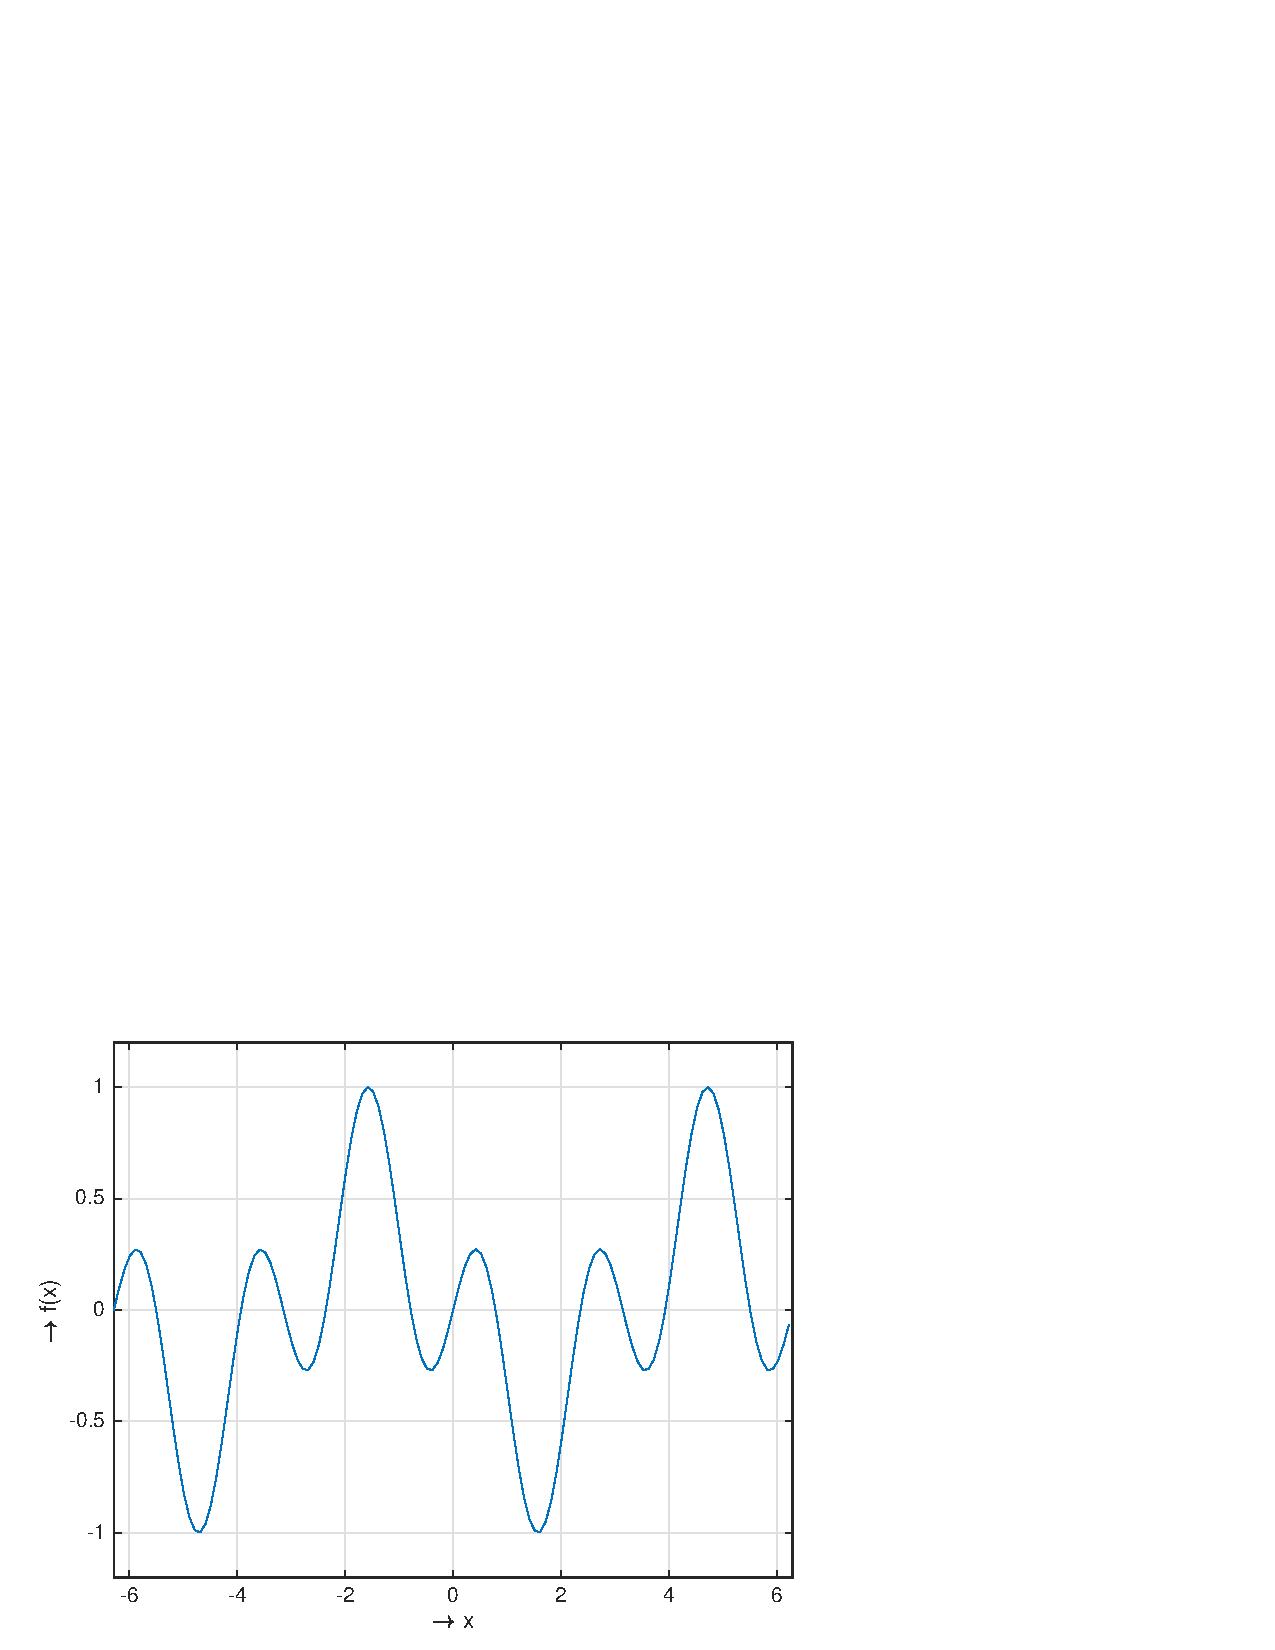
\includegraphics[width=.75\textwidth]{img/sincos}
\caption{Průběh funkce $f(x) = \sin(x)\cos(2x)$}
\label{fig:funcSinCos}
\end{figure}
\end{lstlisting}
%
Výsledek provedení tohoto kódu je vidět na obr. \ref{fig:funcSinCos} na str. \pageref{fig:funcSinCos}.
%
\begin{figure}[ht]
\centering
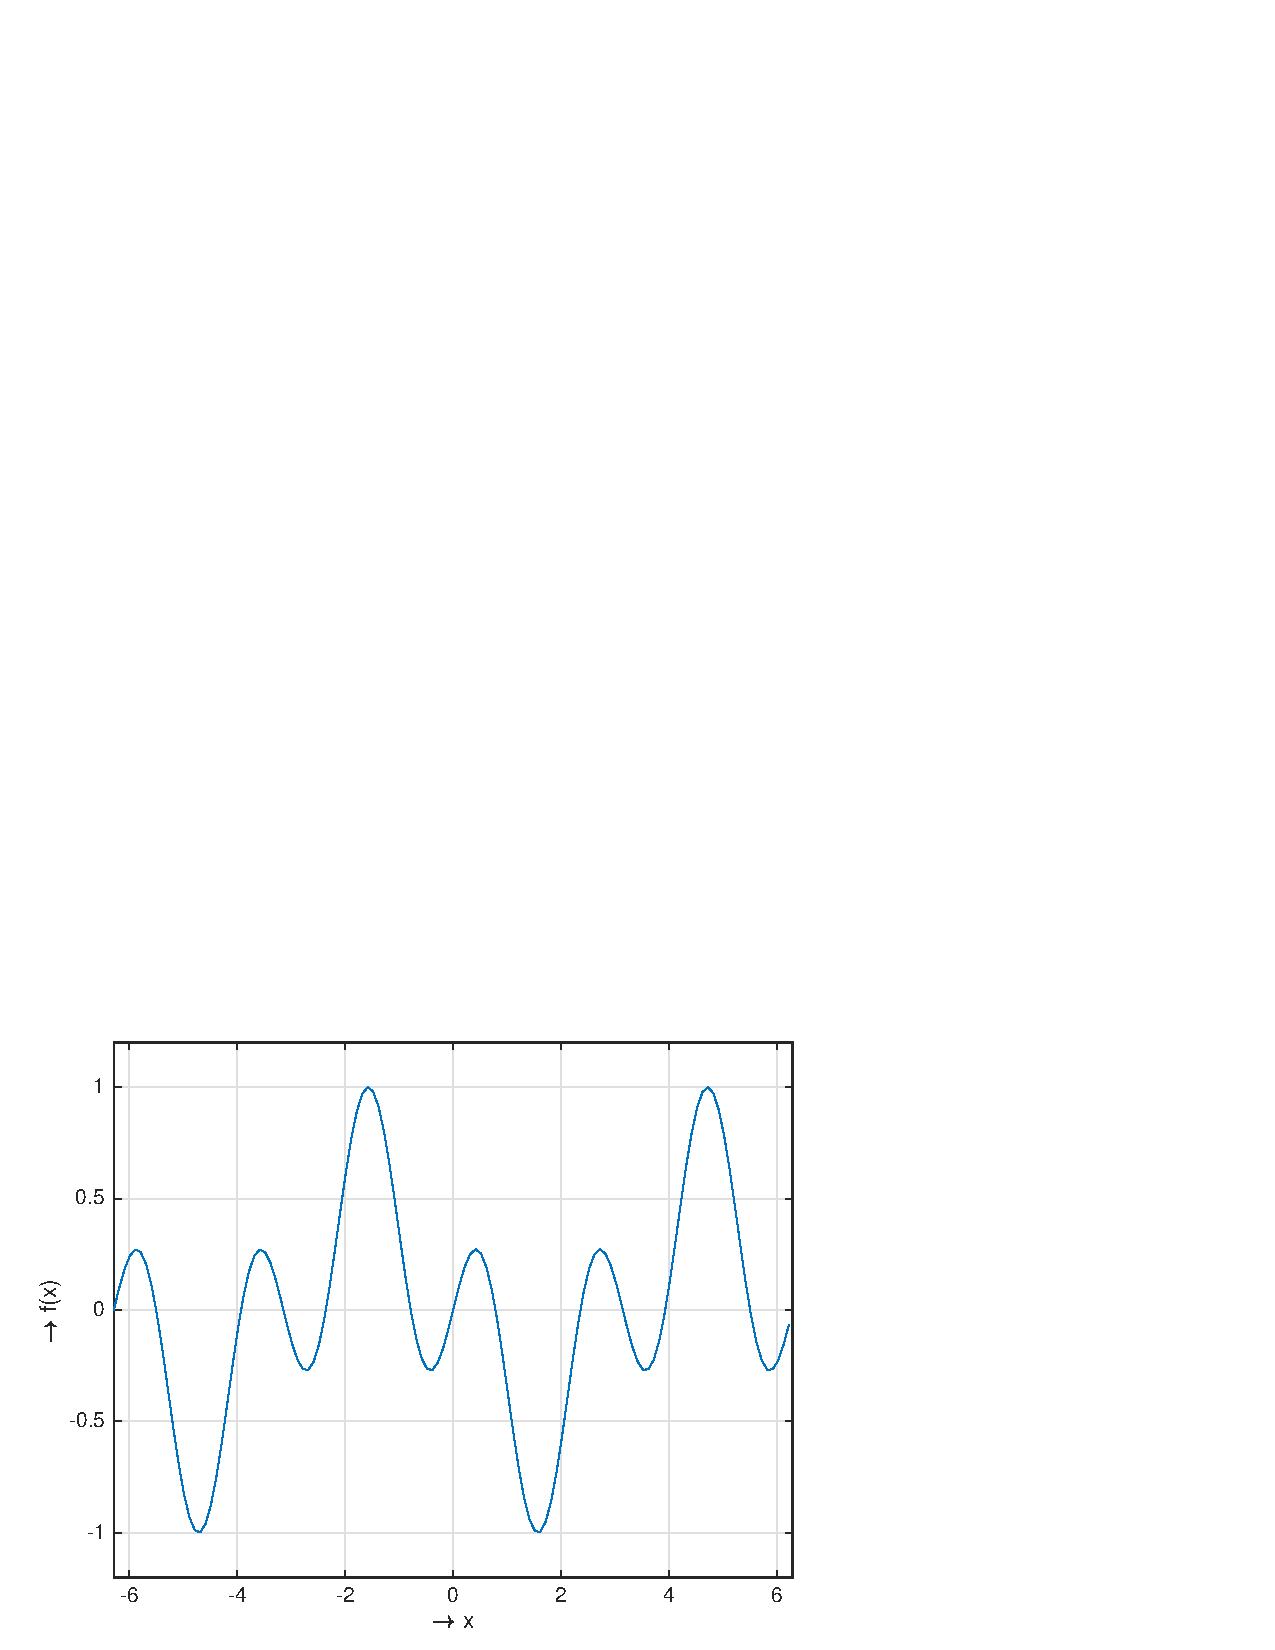
\includegraphics[width=.75\textwidth]{img/sincos}
\caption{Průběh funkce $f(x) = \sin(x)\cos(2x)$}
\label{fig:funcSinCos}
\end{figure}
%
Patrně nejdůležitější věc při vkládání obrázků do dokumentů sázených \TeX{}em je jejich formát.
\begin{important}
Vždy, když je to jen trochu možné, dáváme přednost použití grafiky ve \term{vektorovém formátu}. Rastrovou (bitmapovou\footnote{Ta ale nemusí být nutně uložena jen v~souboru s~příponou \texttt{.bmp}, ale také \texttt{.jpg}, \texttt{.png} atd.}) grafiku užijeme pouze tehdy, kdy z~principu není možné daný grafický motiv uložit ve vektorovém formátu, tedy např. v~případě fotografií či snímků obrazovky. Neexistuje žádný přijatelný důvod pro vkládání rastrové grafiky v~případě grafů funkcí, vývojových či jiných diagramů, schémat, plánů atp.
\end{important}
Je třeba si uvědomit, že tisk (i v~případě starých a nepříliš kvalitních tiskáren) probíhá s~rozlišením minimálně 300 DPI, spíš více. Při tisku v~rozlišení 300 DPI tak rastrová grafika, která má být vytištěná na stránce na šířku textové řádky (tedy asi 13 cm), musí mít horizontálně alespoň 1535 pixelů. Má-li méně, a \TeX{} je i přesto přinucen grafiku roztáhnout na požadovanou velikost, dojde k~viditelnému \uv{rozkostičkování}. U~vektorové grafiky pochopitelně k~tomuto jevu nedochází -- vektorovou grafiku lze zvětšovat/zmenšovat zcela libovolně bez vlivu na kvalitu.
%
\begin{center}
\framebox{\parbox[t]{0.95\textwidth}{Doporučené volně dostupné nástroje pro přípravu ilustrací/grafů/diagramů ve vektorovém formátu jsou např.:\\
\hspace*{1em}(i) \term{yEd} -- \url{https://www.yworks.com/products/yed}\\
\hspace*{1em}(ii) \term{Inkscape} -- \url{https://inkscape.org}\\
\hspace*{1em}(iii) \term{Graphviz} -- \url{https://graphviz.org}\\
\hspace*{1em}(iv) \term{Diagrams.net} -- \url{https://app.diagrams.net}
}}
\end{center}
%
Třída \filename{fasthesis} zavádí (pro vlastní potřebu) balíček \filename{tikz}, který dovoluje vektorovou grafiku vytvářet přímo ve zdrojovém kódu dokumentu pomocí speciálního jazyka geometrických primitiv. Autor dokumentu tedy může tento výkonný nástroj v~případě potřeby okamžitě využít. Níže uvedený kód Shenga Bau~\cite{bau2022} vysadí náhodně vygenerovaný graf zobrazený na obr. \ref{fig:tikzRandomGraph} na str. \pageref{fig:tikzRandomGraph}:
%
\lstset{style=plainsrc}
\begin{lstlisting}
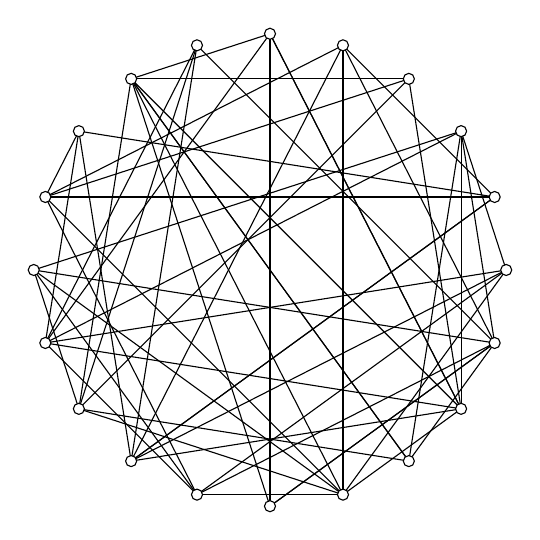
\begin{tikzpicture}
\foreach \i in {0, 1, ..., 19}
{
  \foreach \j in {1, 2, 3} 
  { 
    \pgfmathsetmacro{\thenum}{int(random(0, 19))}
    \draw (18 * \i:3) -- (18 * \thenum:3); 
  } 
} 
\foreach \i in {0, 1, ..., 19}
{
  \filldraw [fill=white,draw=black] (18 * \i:3) circle(2pt); 
} 
\end{tikzpicture}
\end{lstlisting}
%
%
\begin{figure}[ht]
\centering
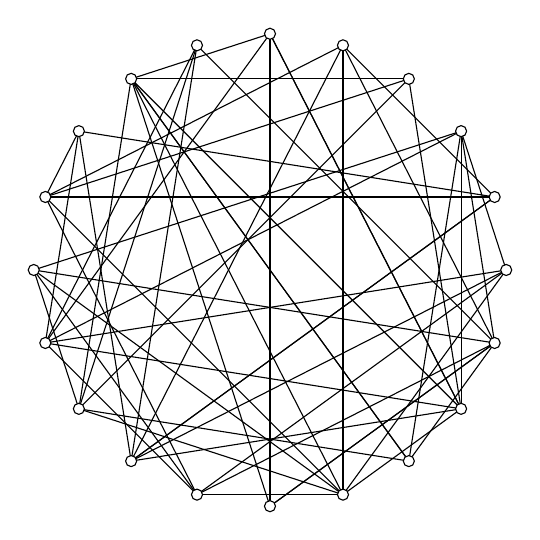
\begin{tikzpicture}
\foreach \i in {0, 1, ..., 19}
{
  \foreach \j in {1, 2, 3} 
  { 
    \pgfmathsetmacro{\thenum}{int(random(0, 19))}
    \draw (18 * \i:3) -- (18 * \thenum:3); 
  } 
} 
\foreach \i in {0, 1, ..., 19}
{
  \filldraw [fill=white,draw=black] (18 * \i:3) circle(2pt); 
} 
\end{tikzpicture}
\caption{Náhodný graf vysazený TikZem podle kódu Shenga Bau~\cite{bau2022}}\label{fig:tikzRandomGraph}
\end{figure}
%
Poslední \textbf{důležitá věc, týkající se sazby obrázků}, ilustrací, grafů apod. je popisek těchto objektů: Tradičně se umisťuje  \textbf{pod} příslušný grafický objekt a obvykle se sází na střed stránky (z~tohoto pravidla lze v~odůvodněných případech činit výjimky). Popisek obrázku začíná velkým písmenem a neukončuje se tečkou. Pokud se popisek skládá z~více vět, pak jsou ukončeny tečkou, nicméně poslední z~nich opět být tečkou ukončena nemusí (je to situace analogická s~nadpisy).
%
%
%
%
\section{Tabulky}
Třída \filename{fasthesis} při své inicializaci zavádí dva užitečné \TeX{}ové balíky \filename"booktabs" a \filename"longtable", které modifikují a doplňují základní možnosti sazby tabulek, nabízené \LaTeX{}em%
\footnote{Podívejte se na jejich dokumentace na webu CTAN (Comprehensive \TeX{} Archive Network) na URL \href{https://ctan.org/pkg/longtable}{\texttt{https://ctan.org/pkg/longtable}}, resp. \href{https://ctan.org/pkg/booktabs}{\texttt{https://ctan.org/pkg/booktabs}}, kde jsou detailně popsány všechny možnosti jejich použití, včetně těch velmi speciálních.}.

Při psaní kvalifikační práce se hodí zejména jedna vlastnost tabulek z~balíku \filename"longtable", a to ta, že tyto tabulky mohou pokračovat přes několik stránek a pomocí příkazů z~balíku lze dokonce specifikovat, jak bude vypadat záhlaví/zápatí nejen v~případě začátku a konce tabulky, ale i v~případě jejího rozdělení na více stránek -- záhlaví/zápatí může být obecně jiné v~případě začátku/konce tabulky a v~případě jejího rozdělení (tj. je např. možné vysázet pod poslední řádek tabulky na jedné straně třeba text \uv{tabulka pokračuje na další straně}, viz tabulka \ref{tab:allclassoptions} na straně \pageref{tab:allclassoptions} tohoto dokumentu).

Jednoduchou tabulku (s~předpřipravenou možností zlomu přes několik stránek) lze vysázet za pomoci příkazů z~balíku \filename"longtable" např. takto:\\
%
\lstset{style=plainsrc}
\begin{lstlisting}
\begin{center}
\begin{longtable}{rr}
\caption{Přehled jednotek množství informace}
\label{tab:infunits}\\
\toprule[1.5pt]
\textbf{jednotka} & \textbf{množství informace}\\
\midrule
\endfirsthead
\multicolumn{2}{c}{\tablename{}~\thetable{}
    \textit{(pokračování z~předchozí stránky)}}\\
\midrule
\textbf{jednotka} & \textbf{množství informace}\\
\midrule
\endhead
\midrule
\multicolumn{2}{r}{%
    \textit{(tabulka pokračuje na další stránce)}}\\
\endfoot
\bottomrule[1.5pt]
\endlastfoot
1 KiB & 1024 B\\
1 MiB & 1048576 B\\
1 GiB & 1073741824 B\\
1 TiB & 1099511627776 B\\
1 PiB & 1125899906842624 B\\
\end{longtable}
\end{center}
\end{lstlisting}
%
Zpracováním výše uvedeného zdrojového kódu vysází \LaTeX{} tabulku v~této podobě:\\
%
\begin{center}
\begin{longtable}{rr}
\caption{Přehled jednotek množství informace}
\label{tab:infunits}\\
\toprule[1.5pt]
\textbf{jednotka} & \textbf{množství informace}\\
\midrule
\endfirsthead
\multicolumn{2}{c}{\tablename{}~\thetable{} \textit{(pokračování z~předchozí stránky)}}\\
\midrule
\textbf{jednotka} & \textbf{množství informace}\\
\midrule
\endhead
\midrule
\multicolumn{2}{r}{\textit{(tabulka pokračuje na další stránce)}}\\
\endfoot
\bottomrule[1.5pt]
\endlastfoot
1 KiB & 1024 B\\
1 MiB & 1 048 576 B\\
1 GiB & 1 073 741 824 B\\
1 TiB & 1 099 511 627 776 B\\
1 PiB & 1 125 899 906 842 624 B\\
\end{longtable}
\end{center}
%
Pochopitelně, že tahle tabulka rozdělená přes více stránek není (protože je na to moc krátká), ale ze zdrojového kódu je patrné, jak pomocí příkazů \verb"\endfirsthead", \verb"\endhead", \verb"\endfoot" a \verb"\endlastfoot" \uv{vysvětlit} \TeX{}u, jak vypadá první a všechna další záhlaví tabulky, resp. poslední zápatí a všechna předchozí před tímto posledním. Tabulka se tedy může lámat přes více stránek: Na začátku je použita definice záhlaví končící příkazem \verb"\endfirsthead", na další stránce pak bude tabulka začínat opět záhlavím, ale tentokrát podle definice ukončené příkazem \verb"\endhead". Analogicky to funguje pro zápatí. Detaily na URL \href{https://ctan.org/pkg/longtable}{\texttt{https://ctan.org/pkg/longtable}}.
\begin{important}
Povšimněte si, prosím, že u~tabulek (a také třeba u~výpisů zdrojového kódu) se ve shodě s~tradičními pravidly sazby \textbf{umisťuje popisek nad příslušnou tabulku}.
\end{important}
%
%
%
%
\section{Zdrojový kód}
Třída dokumentu \filename"fasthesis" využívá pro sazbu zdrojového kódu balík \filename"listings", který se automaticky
připojí, jakmile šablonu použijete. Je tedy možné v~textu přímo používat příkazy a prostředí, které balík \filename"listings"
poskytuje, zejména tedy prostředí \command"lstlisting", přičemž vzhled výsledného výpisu kódu se nastavuje pomocí
příkazů \verb"\lstdefinestyle{"\textsl{mujstyl}\verb"}{"\dots\verb"}" a \verb"\lstset{style="\textsl{mujstyl}\verb"}".

Šablona dává uživateli k~dispozici styl výpisu zdrojového kódu pojmenovaný ``\verb"FASThesisLstStyle"'' (vzhled odpovídá tomu v~ukázce zdrojového kódu \ref{lst:demosrc} na str. \pageref{lst:demosrc}). Autor tedy může tento předpřipravený styl využít a ručně pak třeba dodefinovat další požadované vlastnosti výpisu zdrojového kódu, např. takto:
%
\lstset{style=plainsrc}
\begin{lstlisting}[mathescape=true]
\lstset{style=FASThesisLstStyle, numberblanklines=false,
        tabsize=5, keywordstyle=\color{red}}
\begin{lstlisting}
...
\$$end{lstlisting}
\end{lstlisting}
%
Řídíme-li si sazbu zdrojového kódu vlastními silami, je třeba jen mít na paměti, že výpis \textbf{musí být opatřen popiskem} s číslem výpisu -- tento popisek se sází nad samotným výpisem (tak jako je to na ukázce \ref{lst:demosrc}). Je to proto, aby bylo možné se na kód z textu práce odkazovat. Ze stejného důvodu \textbf{musí být řádky výpisu číslované}. Odkazování z textu pak vypadá např. takto: \uv{\dots typické použití popsané konstrukce lze vidět na ř. 2 zdrojového kódu \ref{lst:demosrc} na str. \pageref{lst:demosrc}.}

Pro méně zdatné uživatele \LaTeX{}u je v~definici třídy pomocí balíku \filename"listings" připraveno prostředí \command"code", které se používá např. takto:
%
\lstset{style=plainsrc}
\begin{lstlisting}
\begin{code}{C}{Ukázkový výpis kódu v~jazyce ANSI C}
int fact(int n) {
	if (n <= 0)
		return 1; /* protože 0! = 1 */
	else
		return n * fact(n - 1);
}
\end{code}
\end{lstlisting}
%
Vysázený výpis zdrojového kódu v~dokumentu pak vypadá takto:
\begin{code}{C}{Ukázkový výpis kódu v~jazyce ANSI C\label{lst:demosrc}}
int fact(int n) {
	if (n <= 0)
		return 1; /* protože 0! = 1 */
	else
		return n * fact(n - 1);
}
\end{code}
%
Pokud se z~textu na zdrojový kód odkazuje, je nutné umístit \textbf{za} popisek cílové návěstí odkazu příkazem \verb"\label{"\textsl{identifikátor návěstí}\verb"}". V~případě výpisu zdrojového kódu se identifikátoru návěstí obvykle předřazuje prefix ``\verb"lst"'':
%
\lstset{style=plainsrc}
\begin{lstlisting}
\begin{code}{C}{Výpočet faktoriálu v~C\label{lst:faktorial}}
...
\end{code}
\end{lstlisting}
%
Seznam všech výpisů zdrojových kódů (a také všech výpisů obsahu konzole, viz část \ref{sec:console}) se vygeneruje příkazem \verb"\listoflistings", který patří do části dokumentu zvané \term{back matter}, tedy na konec práce, za bibliografii, spolu s~případným seznamem obrázků, tabulek, vzorců, indexem atp.
%
%
%
%
\section{Terminál/konzole operačního systému}\label{sec:console}
Máloco vypadá v~sazbě kvalifikačních a podobných prací (a obecně technických dokumentů) tak špatně, jako nekvalitní screenshot \term{konzole} -- nebo chcete-li terminálu či příkazového řádku -- operačního systému (totéž platí pochopitelně pro terminálový přístup k~serveru).

Prakticky všechny operační systémy hlavního proudu používají (patrně z~historických důvodů) v~terminálech černou (nebo jinou velmi tmavou barvu) pro pozadí a bílou (nebo jinou světlou) barvu pro text. Toto v~kombinaci s~výrazně nižší hustotou bodů monitorů\footnote{Monitor má typicky rozlišení od 72 PPI v~případě starých kusů s~malým množstvím pixelů (z~dnešního pohledu) po zhruba 200 u~špičkových moderních tzv. HiDPI monitorů grafických pracovních stanic. Ovšem tisk na laserové tiskárně (i docela staré) začíná na 300 DPI\dots} než mají běžné laserové tiskárny, a také s~faktem, že řada terminálových aplikací stále používá \uv{staré} rastrové fonty, vede většinou k~nepřijatelnému výsledku: Na půlce stránky je černý obdélník (tj. obrovská a zcela zbytečná spotřeba toneru), na kterém jsou nepřirozeně velká, \uv{zubatá}, rozkostičkovaná písmena, často ještě v~důsledku uložení do formátu JPEG notně poškozená artefakty ztrátové komprese.

Třída dokument \filename"fasthesis" proto nabízí autorům prací prostředí \command"console", které dovoluje vysázet výpisy v~terminálu/konzoli operačního systému \uv{kulturně}. Zda půjde o~příkazový řádek operačního systému Windows nebo o~terminál unix\-ové\-ho systému, se rozlišuje použitím dvou různých tzv. promptů -- \verb"\winprompt" a \verb"\uxprompt".

Ve zdrojovém kódu dokumentu může vypadat použití prostředí \command"console" ve variantě s~windowsovským promptem např. takto:
%
\lstset{style=plainsrc}
\begin{lstlisting}
\setwinprompt{C:/Windows/System32}
\begin{console}{Ukázkový výpis obsahu příkazového
  řádku Windows\label{lst:demoConWin}}
`\winprompt`ipconfig

Windows IP Configuration


Ethernet adapter Ethernet:

   Connection-specific DNS Suffix  . : xyz.net
   Link-local IPv6 Address . . . . . : bc95::1255:cd70:71...
   IPv4 Address. . . . . . . . . . . : 192.168.1.101
   Subnet Mask . . . . . . . . . . . : 255.255.255.0
   Default Gateway . . . . . . . . . : 192.168.1.1

Ethernet adapter Ethernet 2:

   Connection-specific DNS Suffix  . :
   Link-local IPv6 Address . . . . . : aa71::c21d:2cf8:25...
   IPv4 Address. . . . . . . . . . . : 192.168.56.1
   Subnet Mask . . . . . . . . . . . : 255.255.255.0
   Default Gateway . . . . . . . . . :

`\winprompt`
\end{lstlisting}
%
Příkaz \verb"\setwinprompt{"\textsl{aktivní složka}\verb"}" nastavuje aktivní složku, ve které se uživatel právě nachází a kde zadává příkazy, a která je tak součástí promptu. Při použití tohoto příkazu se aktivní složka (nebo chcete-li \emph{cesta} čili \emph{path}) zapisuje s~normálními lomítky jako oddělovači složek, nikoliv se zpětnými. Je to proto, že zpětné lomítko uvozuje příkazy \TeX{}u. Každopádně vysázené to bude správně se zpětnými lomítky, tak jak to v~operačním systému Windows má být -- příkaz \verb"\setwinprompt" si normální lomítka sám převede na zpětná.

Vysázení promptu zajistí příkaz \verb"\winprompt", který by ovšem \TeX{} ignoroval (protože je uvnitř prostředí pro doslovný výpis), takže je nutné ho tzv. \term{escapovat}, tedy v~tomto konkrétním případě uzavřít do zpětných apostrofů, což \TeX{}u říká: \uv{Tento příkaz nesázet, ten provést!}

Vysázený výpis příkazu a jeho výstupu z~ukázky výše v~příkazovém řádku operačního systému Windows pak vypadá takto:
\setwinprompt{C:/Windows/System32}
\begin{console}{Ukázkový výpis obsahu příkazového řádku Windows\label{lst:demoConWin}}
`\winprompt`ipconfig

Windows IP Configuration


Ethernet adapter Ethernet:

   Connection-specific DNS Suffix  . : xyz.net
   Link-local IPv6 Address . . . . . : bc95::1255:cd70:711b:223%11
   IPv4 Address. . . . . . . . . . . : 192.168.1.101
   Subnet Mask . . . . . . . . . . . : 255.255.255.0
   Default Gateway . . . . . . . . . : 192.168.1.1

Ethernet adapter Ethernet 2:

   Connection-specific DNS Suffix  . :
   Link-local IPv6 Address . . . . . : aa71::c21d:2cf8:252f:8a35%7
   IPv4 Address. . . . . . . . . . . : 192.168.56.1
   Subnet Mask . . . . . . . . . . . : 255.255.255.0
   Default Gateway . . . . . . . . . :

`\winprompt`
\end{console}
%
Obdobně funguje sazba terminálu operačních systému unixového typu. K~nastavení pracovního adresáře\footnote{Teď se jedná o~operační systém unixového typu, a je tedy na místě použít terminologii UNIXu. Ostatně \uv{místo}, kde se uživatel v~hierarchické struktuře souborového systému právě nachází, vypisuje příkaz ``{\ttfamily\footnotesize pwd}'', tedy {\itshape{\bfseries p}rint {\bfseries w}orking {\bfseries d}irectory}.} se v~případě unixového terminálu použije obdobný příkaz \verb"\setuxprompt{"\textsl{uživatelské jméno vč. stroje}\verb"}{"\textsl{pracovní adresář}\verb"}", který má ovšem argumenty 2: (i) název stroje, na kterém uživatel pracuje, kterému obvykle předchází i uživatelské jméno daného uživatele, a (ii) právě používaný, aktivní pracovní adresář, zapisovaný běžným způsobem užívaným v~UNIXu:
%
\lstset{style=plainsrc}
\begin{lstlisting}
\setuxprompt{Kamil@CML}{/usr/bin}
\begin{console}{Ukázkový výpis obsahu terminálu Linuxu
  \label{lst:demoConUx}}
`\uxprompt`ls -la | grep "^.\{48\}a"
-rwxr-xr-x   1 Kamil None    53956 Nov 13 13:03 addftinfo.exe
-rwxr-xr-x   1 Kamil None     3075 Feb 11 20:45 addgnupghome
-rwxr-xr-x   1 Kamil None  1150349 Jan 21 12:58 addr2line.exe
-rwxr-xr-x   1 Kamil None   165785 Nov 13 13:03 afmtodit
-rwxr-xr-x   1 Kamil None    15433 Dec 22 10:05 afslog.exe
-rwxr-xr-x   1 Kamil None    50220 Oct 22 20:23 agetty.exe
-rwxr-xr-x   1 Kamil None     2217 Feb 11 20:45 applygnupg...
-rwxr-xr-x   2 Kamil None  1177671 Jan 21 12:58 ar.exe
-rwxr-xr-x   1 Kamil None    35876 Nov 15 18:07 arch.exe
-rwxr-xr-x   2 Kamil None  1837207 Jan 21 12:58 as.exe
-rwxr-xr-x   1 Kamil None   108312 Jan 24 20:50 ash.exe
-rwxr-xr-x   1 Kamil None    27040 May 14  2022 autopoint
-rwxr-xr-x   1 Kamil None   686902 Dec 16 02:40 awk.exe
`\uxprompt`
\end{console}
\end{lstlisting}
%
Následkem provedení výše uvedeného zdrojového kódu dostaneme toto:
%
\setuxprompt{Kamil@CML}{/usr/bin}
\begin{console}{Ukázkový výpis obsahu terminálu Linuxu\label{lst:demoConUx}}
`\uxprompt`ls -la | grep "^.\{48\}a"
-rwxr-xr-x   1 Kamil None    53956 Nov 13 13:03 addftinfo.exe
-rwxr-xr-x   1 Kamil None     3075 Feb 11 20:45 addgnupghome
-rwxr-xr-x   1 Kamil None  1150349 Jan 21 12:58 addr2line.exe
-rwxr-xr-x   1 Kamil None   165785 Nov 13 13:03 afmtodit
-rwxr-xr-x   1 Kamil None    15433 Dec 22 10:05 afslog.exe
-rwxr-xr-x   1 Kamil None    50220 Oct 22 20:23 agetty.exe
-rwxr-xr-x   1 Kamil None     2217 Feb 11 20:45 applygnupgdefaults
-rwxr-xr-x   2 Kamil None  1177671 Jan 21 12:58 ar.exe
-rwxr-xr-x   1 Kamil None    35876 Nov 15 18:07 arch.exe
-rwxr-xr-x   2 Kamil None  1837207 Jan 21 12:58 as.exe
-rwxr-xr-x   1 Kamil None   108312 Jan 24 20:50 ash.exe
-rwxr-xr-x   1 Kamil None    27040 May 14  2022 autopoint
-rwxr-xr-x   1 Kamil None   686902 Dec 16 02:40 awk.exe
`\uxprompt`
\end{console}
%
%
%
%
\section{Když je něco opravdu hodně důležité}\label{sec:veryImportant}
Třída dokumentu \filename"fasthesis" nabízí autorům kvalifikačních prací zvláštní prostředí pojmenované \command"important", jehož úkolem je \emph{silně graficky akcentovat} určitou část textu, kterou autor považuje za mimořádně důležitou. Ovšem \textbf{pozor, není dobré toto prostředí nadužívat}, protože opticky silně narušuje souvislý tok textu a také nutnost často zvýrazňovat určité pasáže jako mimořádně důležité může znamenat, že autor nemá koncepci textu řádně promyšlenou.

Jak se prostředí \command"important" při sazbě dokumentu používá, ukazuje následující úsek zdrojového kódu:
%
\lstset{style=plainsrc}
\begin{lstlisting}
\begin{important}
Tento text považuje autor práce z~nějakého důvodu za
mimořádně důležitý a je za každou cenu nutné, aby si ho
čtenář povšiml a věnoval mu maximální možnou pozornost.
Toho je dosaženo zmenšením šířky sazby a ve zbylém místě
na okrajích je text výrazně orámován červenou (nebo černou
v~případě nastavení třídy dokumentu \filename"fasthesis"
na černobílou sazbu přepínačem ``\command"prn"'') barvou.
\end{important}
\end{lstlisting}
%
Výsledek vidíte v~následujícím odstavci:
%
\begin{important}
Tento text považuje autor práce z~nějakého důvodu za
mimořádně důležitý a je za každou cenu nutné, aby si ho
čtenář povšiml a věnoval mu maximální možnou pozornost.
Toho je dosaženo zmenšením šířky sazby a ve zbylém místě
na okrajích je text výrazně orámován červenou (nebo černou
v~případě nastavení třídy dokument \filename"fasthesis"
na černobílou sazbu přepínačem ``\command"prn"'') barvou.
\end{important}
%
Je-li z~nějakého důvodu nutné změnit barvu postranních zvýrazňovacích pruhů, je možné tak učinit pomocí aparátu balíčku \filename"xcolor". Příkazem \verb"\definecolor" se změní nastavení barvy pojmenované \verb"FASThesis@ImportantColor". Pokud tedy chce autor namísto předvolené červené zvýrazňovat důležitý text třeba zelenou barvou, učiní to třeba takto:
%
\lstset{style=plainsrc, numbers=none}
\begin{lstlisting}
\definecolor{FASThesis@ImportantColor}{cmyk}{1.0, 0, 1.0, 0}
\end{lstlisting}
%
Netřeba dodávat, že výše uvedený příkaz se musí ve zdrojovém kódu dokumentu objevit \textbf{před} použitím prostředí \command"important"\footnote{Samozřejmě, že pokud se do toho pustíte, musíte také dočasně povolit používání znaku zavináč (``\verb"@"'') jako běžného písmene (příkazy $\backslash$\texttt{makeatletter} a $\backslash$\texttt{makeatother}).}.
%
%
%
%
\section{Užitečné drobnosti}
Třída \filename"fasthesis" dává autorovi k~dispozici ještě několik jednoduchých příkazů pro usnadnění práce (a také pro celkem žádoucí zvýšení podílu sémantické informace v~textu). Výběr těchto pomocných příkazů je pochopitelně poplatný tomu, že primárními uživateli šablony jsou studenti FAV. Pokud zde nenajdete, co hledáte/potřebujete/očekáváte, vzhůru do studia jazyka \TeX{}u a vlastnoručního kódování \TeX{}ových maker (tedy příkazů).

\paragraph{Sazba významných/nově definovaných odborných termínů} K~vyznačení důležitých nebo právě definovaných odborných termínů či zaváděných pojmů lze využít příkaz \verb"\term{"\textsl{termín}\verb"}":
%
\lstset{style=plainsrc, numbers=none}
\begin{lstlisting}
Jako \term{stacionární bod} funkce $f(x)$ označujeme takový
bod $a$ z~jejího definičního obodu, pro který platí, že
$\frac{\mathrm{d}f}{\mathrm{d}x}(a) = 0$.
\end{lstlisting}
%
Následující odstavec ukazuje výsledek po zpracování \LaTeX{}em:\\
\par\noindent
Jako \term{stacionární bod} funkce $f(x)$ označujeme takový
bod $a$ z~jejího definičního obodu, pro který platí, že
$\frac{\mathrm{d}f}{\mathrm{d}x}(a) = 0$.

\paragraph{Sazba názvů souborů či cest v~souborovém systému} Pro tento účel je připraven příkaz \verb|\filename"|\textsl{název souboru}\verb|"|, jehož parametrem je cesta v~souborovém systému (tzv. \term{path}). Sazba zejména cest v~operačním systému Windows je v~\TeX{}u problematická, poněvadž \TeX{} používá jako uvozující znak příkazů zpětné lomítko (``\textbackslash''), které ve Windows slouží jako oddělovač jednotlivých složek v~cestě. Z~toho důvodu není možné vysázet cestu běžným způsobem:
%
\lstset{style=plainsrc, numbers=none}
\begin{lstlisting}
... \texttt{C:\Program Files\System32} ...
\end{lstlisting}
%
Na to reaguje \TeX{} chybovým hlášení, že nezná příkaz \verb"\Program". Řešení nabízí právě příkaz \verb"\filename", jehož použití je naznačeno v~následujícím výpisu zdrojového kódu:
%
\lstset{style=plainsrc, numbers=none}
\begin{lstlisting}
... \filename"C:\Program Files\System32" ...
\end{lstlisting}
%
\textbf{Pozor:} Tento příkaz (z~implementačních důvodů) vyžaduje argument uzavřený mezi dvěma \textbf{stejnými} znaky, nikoliv mezi levou a pravou složenou závorku, jak je to obvyklé. V~roli \uv{závorky} lze použít jakýkoliv znak, který se nevyskytuje v~argumentu, takže např. uvozovky jako v~ukázce nebo třeba znak kůl (``|''), hvězdička, vykřičník atp.; třeba takto \verb"\filename*C:\Program Files\System32*".

\paragraph{Sazba příkazů či krátkých úseků zdrojového kódu} Obdobná situace nastává, je-li třeba vysázet některé úseky zdrojového kódu, které jsou natolik krátké, že nemá smysl je umisťovat do prostředí \command"code" (nebo obdobného na bázi \command"lstlisting"), ale zároveň obsahují znaky, které \TeX{} specifickým způsobem interpretuje. Příkladem může být třeba část kódu v~MATLABu: \command"X = A \ B". Tam se vyskytuje zpětné lomítko, které \TeX{} interpretuje jako uvozující znak příkazu.

K~sazbě takových sekvencí znaků je určen příkaz \verb|\command"|\textsl{zdrojový kód}\verb|"|, v~jehož parametru mohou být i speciální znaky, které by jinak \TeX{} interpretoval. Jeho použití je velmi přímočaré:
%
\lstset{style=plainsrc, numbers=none}
\begin{lstlisting}
... \command"X = A \ B" ...
\end{lstlisting}
%
Opět platí, že roli \uv{závorky}, ve které je argument uzavřen, může hrát jakýkoliv znak, který se pak ale v~argumentu samozřejmě nesmí vyskytovat (a otevírací i uzavírací \uv{závorka} argumentu je stejná).

\paragraph{Sazba názvů či označení (softwarových) produktů} Obecně se považuje za vhodné opatřovat úseky textu dodatečnou sémantickou informací\footnote{Tj. nějak určit, že právě tato sekvence znaků je třeba názvem nějakého produktu.} všude tam, kde je to možné a účelné. Takovou situací může být třeba označování názvů různých výrobků, softwarových (např. \product{Inkscape} nebo \product{ReactOS}) nebo jiných produktů k~tomu určeným příkazem \verb"\product{"\textsl{název produktu}\verb"}", čímž jednak dojde k~jejich zvýraznění v~textu a jednak je možné s~nimi dále pracovat (např. vytvořením jejich seznamu apod.):
%
\lstset{style=plainsrc, numbers=none}
\begin{lstlisting}
Můj oblíbený textový editor \product{Notepad++} se hodí k~...
\end{lstlisting}
%

\paragraph{Sazba \uv{tlačítek}} Při popisu např. grafického uživatelského rozhraní nějaké aplikace nebo třeba webové stránky se může hodit v~textu graficky znázornit tlačítko, na které má uživatel kliknout apod. K~tomu slouží příkaz \verb"\button{"\textsl{text na tlačítku}\verb"}":
%
\lstset{style=plainsrc, numbers=none}
\begin{lstlisting}
Po vyplnění formuláře klikněte na \button{Odeslat}.
\end{lstlisting}
%
Výsledkem výše uvedeného kódu je:
\begin{center}
Po vyplnění formuláře klikněte na \button{Odeslat}.
\end{center}

\paragraph{Sazba kláves a klávesových zkratek} Při popisu ovládání software se často v~dokumentech vyskytují sekvence kláves či jejich kombinací, které je třeba stisknout, aby proběhla požadovaná činnost. Třída \filename"fasthesis" poskytuje k~sazbě stisknutých kláves či jejich kombinací příkaz \verb"\hotkey{"\textsl{označení kláves(y)}\verb"}": %
\lstset{style=plainsrc, numbers=none}
\begin{lstlisting}
Při psaní kvalifikační práce nezapomínejte na \hotkey{Ctrl+S}.
\end{lstlisting}
%
Výsledkem výše uvedeného kódu je:
\begin{center}
Při psaní kvalifikační práce nezapomínejte na \hotkey{Ctrl+S}.
\end{center}
Není to nic světoborného, ale důsledným používáním lze dosáhnout zejména tolik žádoucí (typo)grafické konzistence vytvářeného dokument. Navíc užíváním takovýchto jednoduchých příkazů (klidně si je vytvářejte i sami, je to dobrá věc) systematicky injektujeme další sémantickou informaci do textu (to je za všech okolností žádoucí) a pak třeba jen hledání, kde všude jsou uvedené nějaké klávesové zkratky, je výrazně snazší a rychlejší.

% _____________________________________________________________________________
%
%
%        APPENDICES
%
% _____________________________________________________________________________
%
\appendix
% _____________________________________________________________________________
%
%
%		APPENDIX CHAPTER
%
% _____________________________________________________________________________
%
\chapter{Lokální instalace fontu GT America}\label{app:installgta}
Třída dokumentu \filename"fasthesis.cls" používá font \term{GT America} navržený nezávislou švýcarskou písmolijnou \term{Grilli Type}. Tento font je v~\emph{Manuálu jednotného vizuálního stylu Západočeské univerzity v~Plzni} určen jako jeden ze dvou základních fontů, které vizuální identitu ZČU definují. Font ovšem není součástí instalace \LaTeX{}u a ani pro něj neexistuje \TeX{}ový balíček. Je to proto, že \term{GT America} není volně dostupný -- je třeba k~němu mít licenci (kterou ZČU pochopitelně zakoupila, aby mohla font legálně používat).

Font se tedy musí doinstalovat, aby bylo možné třídu \filename"fasthesis.cls" úspěšně využít k~sazbě dokumentu. Není třeba se toho bát -- \TeX{} se chová velmi \uv{rozumně}, jen je nutné mu pár věcí vysvětlit. Postupujte podle níže uvedeného návodu:
\begin{enumerate}
\item V~instalačním archivu \filename"fasthesis.zip" je podsložka \filename"install" a v~ní pak podsložka
\filename"$TEXMFLOCAL".
Obsah této podsložky (jsou tam dvě složky \filename"fonts" a \filename"tex") je třeba nakopírovat do kořenové složky lokální instalace \TeX{}u (to bývá např. v operačním systému \term{Windows} v případě distribuce MiK\TeX{}u složka \filename"C:\Program Files\MiKTeX").
\item Potom je třeba upravit tzv. \term{mapu fontů}. To se udělá příkazem
``\texttt{initexmf} \verb"--edit-config-file"\hspace{0.5em}\texttt{updmap}'' v konzoli. Je-li \TeX{} nainstalován správně, spus\-tí se po zadání tohoto příkazu předvolený systémový textový editor (v nejhorším případě \term{Notepad}) a v něm se otevře soubor \filename"updmap.cfg" -- tedy konfigurační soubor globální mapy \TeX{}ových fontů. Do tohoto konfiguračního souboru (na konec) musíme připsat řádek ``\verb"Map GTAmerica"''.
\item Po úpravě konfigurace mapy fontů je nutné celou mapu přegenerovat příkazem ``\verb"initexmf --mkmaps"''.
\item Pro jistotu ještě spustíme program \filename"updmap", který obnoví (přegeneruje) globální mapu fontů, příkazem ``\verb"updmap --verbose"''.
\end{enumerate}
% _____________________________________________________________________________
%
%
%		APPENDIX CHAPTER
%
% _____________________________________________________________________________
%
\chapter{Přehled balíčků importovaných třídou {\ttfamily fasthesis}}
Třída dokumentu \filename{fasthesis} využívá (a tedy během své instanciace úvodním příkazem dokumentu \verb"\documentclass["\textsl{\dots}\verb"]{fasthesis}" zavádí) níže popsané \LaTeX{}ové balíčky:
\begin{enumerate}
\item\texttt{memoir} -- třída dokumentu, od které je třída naší šablony \filename{fasthesis} odvozena. Jedná se o velmi \uv{mocnou} třídu, která nahrazuje starší třídy \LaTeX{}u 2.09$\mathrm{\epsilon}$ \texttt{article}/\texttt{report}/\texttt{book}.
\item\texttt{inputenc} -- zajišťuje správnou interpretaci znaků z rozšířených znakových sad (CP-1250, UTF-8 atp.) ve zdrojovém kódu dokumentu \LaTeX{}em.
\item\texttt{fontenc} -- zajišťuje správné mapování znaků ve zdrojovém kódu dokumentu na \emph{typy} (\emph{písmové znaky}) použitého fontu.
\item\texttt{newtx} -- balíček, umožňující \LaTeX{}u využívat fonty z projektu \emph{TX Fonts}, tedy volně dostupné virtuální fontu odvozené od fontu \emph{Adobe Times} a upravené pro \LaTeX{}.
\item\texttt{newtxmath} -- viz předchozí, varianta pro sazbu matematických symbolů.
\item\texttt{microtype} -- balíček tzv. \emph{mikrotypografických} rozšíření, jejichž aplikaci v dokumentu umožnilo široké rozšíření pdf\LaTeX{}u. Dovoluje dokonale \uv{vyladit} sazbu použitým fontem např. adaptivním prostrkáním, rozpalem apod.

\item\texttt{babel} -- rozsáhlý balíček podpory cizích jazyků (tedy např. češtiny, která je normálně \LaTeX{}u dost cizí).
\item\texttt{csquotes} -- korektivní balíček zajišťující správnou sazbu českých uvozovek, tedy těch, jejichž uvozující znak leží na účaří a ukončující na horní dotažnici: \uv{\dots}.
\item\texttt{biblatex} -- balíček pro sazbu bibliografických informací na konci dokumentu a správu citací v~textu.

\item\texttt{graphicx} -- rozsáhlý a velmi \uv{mocný} balíček pro vkládání grafických objektů do dokumentu a manipulaci s~nimi.
\item\texttt{xcolor} -- balíček pro práci s~barvami; umožňuje jednak barvy definovat v~několika různých barevných prostorech a následně jimi obarvovat jednotlivé komponenty sazby (text, pozadí aj.).
\item\texttt{eso-pic} -- balíček, který dovoluje vkládat grafické motivy na pozadí stránek.
\item\texttt{tcolorbox} -- balíček, jehož pomocí lze obarvovat tzv. \emph{boxy}, tedy sesazené (ohraničené nebo neohraničené) pravoúhlé oblasti naplněné textem.
\item\texttt{qrcode} -- balíček, který umožňuje sázet QR kódy různých typů; v~šabloně je využit pro (nepovinné)
vysazení QR kódu s~URL práce v~informačním systému STAG na zadní stranu desek/přebalu.

\item\texttt{geometry} -- balíček, který se mění resp. upravuje či přizpůsobuje geometrie stránky a tzv. \emph{sazebné zrcadlo}, tedy např. vzdálenosti textu od okrajů, velikosti záhlaví a zápatí apod.

\item\texttt{tikz} -- mohutný balík pro tvorbu a následnou sazbu vektorových ilustrací; pomocí speciálního jazyka na základě geometrických primitiv dovoluje popsat vzhled grafického motivu a ten posléze vložit do dokumentu.

\item\texttt{hyperref} -- balíček, kterým se realizuje sazba aktivních hypertextových odkazů a také specifické typografické provedení jejich URL adres.

\item\texttt{titlesec} -- balíček, s~jehož pomocí lze upravit grafické provedení nadpisů jednotlivých částí dokumentu (kapitol, sekcí, podsekcí atp.).

\item\texttt{listings} -- balíček s~nástroji pro sazbu výpisů zdrojového kódu v~mnoha různých programovacích jazycích, zvýrazňování syntaxe těchto jazyků apod.

\item\texttt{xparse} -- balíček se sadou maker pro syntaktickou analýzu zdrojového kódu v~jazyce \TeX{}u; třída \filename{fasthesis} ho používá k~realizaci některých maker, jejichž parametrem může být řetězec, obsahující znaky se speciálním významem, které by \TeX{} za normálních okolností nějak interpretoval (jako třeba zpětné lomítko).
\item\texttt{xstring} -- balíček, pomocí kterého lze manipulovat s~řetězci (obsahem proměnných, těly maker apod.). Lze např. (i) zjišťovat, zda řetězec začíná nebo končí nějakým znakem, (ii) zkoumat, zda řetězec obsahuje nějaký podřetězec atp.
\item\texttt{booktabs} -- balíček, dovolující sázet komplikovanější a sofistikovanější tabulky, lépe a snáze než to lze standardními prostředky \LaTeX{}u.
\item\texttt{longtable} -- viz předchozí, dovoluje tabulku rozdělit na více stránek.
\end{enumerate}
Detailní informace ke všem balíčkům lze načerpat z~jejich (obvykle velmi podrobných) dokumentací, které se všechny nachází v~archivu zvaném \term{CTAN}, tedy \term{Comprehensive \TeX{} Archive Network}, na adrese URL \url{https://www.ctan.org}.

\begin{important}
Autor dokumentu využívajícího šablonu \filename"fasthesis" může tedy okamžitě a bez zavádění výše popsaných balíčků příkazem \verb"\usepackage" do textu vkládat veškeré příkazy, které tyto balíčky poskytují.
\end{important}
% _____________________________________________________________________________
%
%
%		APPENDIX CHAPTER
%
% _____________________________________________________________________________
%
\chapter{Často kladené dotazy (FAQ)}
\textbf{Proč má výsledný dokument při použití této šablony dvě titulní stránky, jednu barevnou a jednu černobílou? ---}
Protože ta první \uv{titulní strana} vlastně není titulní strana: Je to přední strana desek (nebo chcete-li přebalu). Současné technické možnosti maloprodukční vazby knih bez problémů dovolují je opatřovat plnobarevnými laminovanými deskami, které se mi zdají mnohem hezčí, než ty prastaré látkové či koženkové desky, do kterých se kvalifikační práce vkládaly již za Rakouska-Uherska. Proto šablona vytváří dokument tak, aby měl arch desek/přebalu, tj. přední a zadní stranu, plnobarevnou (příp. i s~grafickým motivem) a autor si tak mohl nechat práci svázat do moderních plnobarevných desek.

Kdo o~tuto variantu nestojí, prostě první a poslední stránku dokumentu (i) zahodí v~případě, že je dokument již vytištěný, nebo (ii) vymaže v~nějakém nástroji pro práci s~dokumenty ve formátu PDF (třeba \product{Adobe Acrobat}, \product{PDF24}, nebo třeba jen terminálový \product{pdftk}).\\
%
%
%
\par\noindent
\textbf{Proč je v~dokumentu tolik prázdných stránek? ---}
Protože je primárně určen k~tisku a svázání. Některé archy jsou ve vázané publikaci potištěné jen z~jedné strany (např. titulka, patitul atp.) a konzervativní pravidla sazby také předepisují, že např. kapitola vždy začíná na liché (tedy při pohledu na otevřenou knihu) pravé stránce. Proto musejí být ve výsledném PDF prázdné stránky na těch pozicích, které jsou opačnými stranami archů potištěných jen z~jedné strany.

Pokud hodláte dokument číst pouze v~elektronické podobě a nebudete ho tisknout, jsou tyto prázdné stránky pochopitelně zbytečné. V~takovém případě se jich lze snadno zbavit použitím přepínače ``\verb"viewonly"'' v~inicializačním příkazu \verb"\"{\ttfamily do\-cu\-ment\-class} -- detaily najdete v~tabulce \ref{tab:allclassoptions} na str. \pageref{tab:allclassoptions}.\\
%
%
%
\par\noindent
\textbf{Proč při překladu \uv{vyskáče} tolik varování, underfull a overfull boxů apod.? ---} Protože grafické provedení sázeného dokumentu definované touto šablonou je (na standardy \TeX{}u) velmi komplexní. Je zde celá řada tabulek, obrázků, výpisů zdrojového kódu atp., takže \TeX{}ovský algoritmus, který skládá boxy na stránku, se dostává často na hranici svých možností a prostě se mu nedaří sesadit boxy lépe, tak aby skóre \uv{ohavnosti} bylo dostatečně nízké. Proto také trochu \uv{nadává}\dots Nicméně to není jakosti výsledku příliš na závadu. Nenechte se tím rozhodit.\\
%
%
%
\par\noindent
\textbf{Šablona obsahuje chyby! Použil jsem příkaz \texttt{$\backslash$xyz} a \TeX{} jen vyházel spoustu chybových hlášek! ---} Šablona byla před zveřejněním velmi intenzivně a velmi důkladně testována. Samozřejmě, že i tak mohla nějaká záludná chyba uniknout mé pozornosti (v~takovém případě mne neváhejte kontaktovat), ale není to příliš pravděpodobné. Zkuste nejprve pořádně prohlédnout svůj kód, zda jste například nezapomněli u~příslušného příkazu uvést některý z~jeho povinných parametrů, zda jste nezapomněli někde uzavírací složenou závorku, zda jsou všechna prostředí začínající příkazem \verb"\begin{"\dots\verb"}" také ukončena odpovídajícím příkazem \verb"\end{"\dots\verb"}" apod.
% _____________________________________________________________________________
%
%
%        BACK MATTER (BIBLIOGRAPHY, LISTS, ...)
%
% _____________________________________________________________________________
%
\backmatter
\printbibliography
\listoffigures
\listoftables
\listoflistings
% _____________________________________________________________________________
%
%		BACK COVER
% _____________________________________________________________________________
%
%\setbackpagepic{img/fav} % <== an example of one possible option (read this manual)
%\setqrcodebaseurl{https://mycloud.org/show=pdf&docid=} % <== another example
%\setbackpageqrcode{54321} % <== and one more (uncomment the one that makes sense for you)
\setbackpageqrcode
\backpage
\end{document}